\documentclass[12pt,a4paper]{article}

\usepackage[margin=1in]{geometry}
\usepackage{graphicx}
\usepackage{setspace}
\usepackage{times}
\usepackage{titlesec}
\usepackage{amsmath, amssymb, amsthm}
\usepackage{booktabs}
\usepackage{array}
\usepackage[pdfpagelabels,plainpages=false]{hyperref}
\hypersetup{hypertexnames=false}
\usepackage{enumitem}
\usepackage{fancyhdr}
\usepackage{indentfirst}
\usepackage{xcolor}
\usepackage{listings}

\hypersetup{
    colorlinks=true,
    linkcolor=black,
    citecolor=black,
    urlcolor=blue
}

\onehalfspacing
\setlength{\parindent}{0.5in}
\setlength{\parskip}{0pt}

\titleformat{\section}
    {\normalfont\bfseries\large}{\thesection.}{0.5em}{}
\titleformat{\subsection}
    {\normalfont\bfseries}{\thesubsection.}{0.5em}{}

\pagestyle{fancy}
\fancyhf{}
\setlength{\headheight}{14.5pt}  % fixes fancyhdr warning in the template
\fancyhead[L]{Neural-Network Classification of Breast FNA Features}
\fancyhead[R]{\thepage}
\renewcommand{\headrulewidth}{0.4pt}

% ---- Title page metadata ----
\newcommand{\UniversityName}{Bulacan State University}
\newcommand{\CollegeName}{College of Science}
\newcommand{\CourseCode}{MCS 306}
\newcommand{\CourseDescription}{Introduction to Artificial Intelligence}
\newcommand{\AcademicYear}{First Semester, Academic Year 2026--2027}
\newcommand{\StudyTitle}{Neural-Network Classification of Breast Fine-Needle-Aspirate Features: A From-Scratch Multilayer Perceptron on the Wisconsin Diagnostic Dataset}
\newcommand{\AuthorNames}{Ardiel Drew L. Cristobal, Eunice Angeline Y. Cruz, Kerby C. Denilla, Carl Louise P. Martin, and Yangel Mica P. Nicolas}
\newcommand{\CourseYearSection}{BSM CS 3A}
\newcommand{\InstructorName}{Aarhus M. Dela Cruz, LPT, MSc}
\newcommand{\SubmissionDate}{November 1, 2026}

% Logo file paths
\newcommand{\BulSULogo}{assets/bulsu.png}
\newcommand{\COSLogo}{assets/college_of_science.png}

% Code listings
\lstset{basicstyle=\ttfamily\footnotesize, breaklines=true, frame=single, numbers=left, numberstyle=\tiny}

\begin{document}

\begin{titlepage}
    \centering

    \vspace*{0.3in}

    \begin{minipage}{0.22\textwidth}
        \centering
        \includegraphics[width=0.95\linewidth]{\BulSULogo}
    \end{minipage}
    \hfill
    \begin{minipage}{0.50\textwidth}
        \centering
        {\Large\bfseries \UniversityName\par}
        \vspace{0.15cm}
        {\large\bfseries \CollegeName\par}
        \vspace{0.15cm}
        {\normalsize \CourseCode: \CourseDescription\par}
        \vspace{0.15cm}
        {\normalsize \AcademicYear\par}
    \end{minipage}
    \hfill
    \begin{minipage}{0.22\textwidth}
        \centering
        \includegraphics[width=0.95\linewidth]{\COSLogo}
    \end{minipage}

    \vspace{1.5in}

    {\Large\bfseries MINI RESEARCH AND EXPOSITION PAPER\par}

    \vspace{0.6in}

    {\Large\bfseries \StudyTitle\par}

    \vspace{0.9in}

    {\large\bfseries Authors\par}
    \vspace{0.2cm}
    {\large \AuthorNames\par}

    \vspace{0.6in}

    {\large \CourseYearSection\par}

    \vfill

    {\normalsize Submitted to:\par}
    \vspace{0.15cm}
    {\normalsize\bfseries \InstructorName\par}

    \vspace{0.4in}

    {\normalsize \SubmissionDate\par}
\end{titlepage}

\pagenumbering{roman}
\setcounter{page}{1}

\begin{abstract}
\noindent This paper studies the classification of breast masses as malignant or benign from 30 numeric features of digitized fine-needle-aspirate images (Breast Cancer Wisconsin (Diagnostic) dataset, 569 examples). We implement a multilayer perceptron with one tanh hidden layer and a sigmoid output from scratch in NumPy, with binary cross-entropy, a weight penalty, backpropagation and full-batch gradient descent. The analytic gradients agree with centered finite differences to within $2.1\times10^{-11}$. With a stratified 70/15/15 split and standardization fitted on the training data only, the learning rate, hidden width and regularization strength $\lambda$ are chosen jointly from a 27-cell grid by the mean validation loss over ten initialization seeds. Without regularization the validation loss rises as the learning rate grows, which is consistent with overfitting. The selected network (learning rate 0.01, 16 hidden units, $\lambda=0.01$) lies on the grid edge on all three axes and stopped at the 5000-epoch cap with a final gradient norm of 0.015658. On the 86 held-out test examples it reaches an accuracy of 0.9884, a precision of 1.0 and a recall of 0.9688, missing one malignant case; its test log loss is 0.0497. Logistic regression makes the same single error (log loss 0.0610), and a majority-class rule reaches an accuracy of 0.6279. No advantage of the multilayer perceptron over logistic regression is observed on this split. The model is educational, not a diagnostic tool.

\noindent\textbf{Keywords:} multilayer perceptron, backpropagation, gradient descent, binary classification, breast cancer diagnosis data
\end{abstract}

\newpage
\tableofcontents
\newpage

\pagenumbering{arabic}
\setcounter{page}{1}

\section{Introduction}
\label{sec:intro}

Breast cancer is a major public-health concern: it caused an estimated 694\,000 deaths worldwide in 2024 and was the most common cancer in women in 164 of 186 countries that year~\cite{who2026}. When a breast mass is found, one way to obtain material for diagnosis is fine-needle aspiration, a minimally invasive diagnostic method~\cite{yu2012}. Telling malignant from benign masses matters because most breast lumps are not cancer, and breast cancers are more likely to be treated successfully when they are small and have not spread to nearby lymph nodes~\cite{who2026}. Interpreting aspirates is not perfectly reproducible between observers: in a retrospective review of 70 breast aspirates read by three experienced cytopathologists, the overall agreement between observers on the five reporting categories was 70.48\%~\cite{boler2022}. This motivates measuring the nuclei quantitatively from digitized images. Street et al.~\cite{street1993} followed this approach: they extracted size, shape and texture features of cell nuclei from digitized aspirate images and classified the samples automatically. The features of 569 such samples are published as the Breast Cancer Wisconsin (Diagnostic) dataset~\cite{wdbc}, which we use.

We use the features here only to study a learning pipeline. The dataset is small, public and well documented, so every step of a learning pipeline can be implemented, run many times and checked. This makes it suitable for an educational study, in which the question is less how high a score can be pushed than how a model is trained, validated and judged honestly.

A multilayer perceptron (MLP) is a relevant model for this task. With no hidden layer and a sigmoid output it reduces to logistic regression, so it contains the standard linear model as a special case; a hidden layer with a nonlinear activation adds the ability to represent nonlinear decision boundaries, and without the nonlinearity the extra layer would add nothing (Section~\ref{sec:prelim-mlp}). The MLP is trained by gradient descent with the gradient computed by backpropagation, whose derivation, implementation and verification are a central part of this paper. Its behavior depends on the learning rate, the width of the hidden layer and the regularization strength, which makes it a good object for studying convergence and for practicing validation-based model selection.

\subsection{Objectives of the Paper}
\label{sec:objectives}

The paper has four objectives, each matched by a part of Section~\ref{sec:results}.
\begin{enumerate}[label=\textbf{O\arabic*.}, leftmargin=*]
  \item Derive backpropagation for a multilayer perceptron with a sigmoid output and binary cross-entropy, implement it from scratch in NumPy, and verify it with a finite-difference gradient check (Sections~\ref{sec:prelim} and~\ref{sec:impl}).
  \item Study how training depends on the learning rate, the hidden width and the regularization strength, selecting the configuration with validation data only (Section~\ref{sec:results}).
  \item Compare the selected network with a logistic regression and a majority-class baseline on a held-out test set (Section~\ref{sec:results}).
  \item Interpret the results and state their limits (Section~\ref{sec:analysis}).
\end{enumerate}

\paragraph{Scope and limitations.}
The study uses a single dataset of 569 samples and one fixed split, with no external validation. The network has one hidden layer, and the training is full-batch gradient descent. The model is an educational classifier, not a diagnostic tool, and the paper makes no clinical claim. Section~\ref{sec:prelim} fixes the notation and derives the required results, Section~\ref{sec:methods} describes the model, its implementation, the results and their analysis, and Section~\ref{sec:concl} concludes with possible extensions.

\section{Preliminaries}
\label{sec:prelim}

This section fixes the notation and states or derives every result used in Section~\ref{sec:methods}. Symbols are plain (non-bold), vectors are column vectors, the example index is the superscript $(r)$, and $\ell$ denotes only the layer index.

\subsection{Supervised binary classification and empirical risk}
\label{sec:prelim-erm}

A labeled dataset $\mathcal{D}=\{(x^{(r)},y^{(r)})\}_{r=1}^{N}$ consists of feature vectors $x^{(r)}\in\mathbb{R}^{d}$ and labels $y^{(r)}\in\{0,1\}$; in this paper $y=1$ denotes a malignant mass and $y=0$ a benign one. A model with parameter vector $\theta\in\mathbb{R}^{P}$ maps $x$ to $\hat p\in(0,1)$, an estimate of $P(y=1\mid x)$, and a hard label is obtained by comparing $\hat p$ with a threshold. A loss function $\mathcal{L}(y,\hat p)\ge 0$ measures the cost of the prediction $\hat p$ when the label is $y$. The empirical risk is the mean loss on the data,
\begin{equation}
  \widehat{R}(\theta)=\frac{1}{N}\sum_{r=1}^{N}\mathcal{L}\bigl(y^{(r)},\hat p^{(r)}\bigr).
  \label{eq:emprisk}
\end{equation}
Training minimizes $\widehat{R}$ plus a regularizer (Section~\ref{sec:prelim-reg}). The quantity of interest, however, is the loss on examples not used for training, which is why the data are split (Section~\ref{sec:prelim-split}).

\subsection{Perceptron and multilayer perceptron}
\label{sec:prelim-mlp}

A perceptron computes a weighted sum of its inputs and applies a hard threshold,
\begin{equation}
  z=Wx+b,\qquad a=\mathbf{1}[z\ge 0],
  \label{eq:perceptron}
\end{equation}
with $W\in\mathbb{R}^{1\times d}$ and $b\in\mathbb{R}$. The threshold function is constant on $z<0$ and on $z>0$, so its derivative is zero wherever it exists; a gradient of a loss with respect to $W$ and $b$ therefore carries no information. Replacing the threshold by a smooth activation function $\phi$ removes this obstacle and allows gradient-based training.

A multilayer perceptron (MLP) with $L$ parameterized layers composes such units. With $a^{[0]}=x$ and $\ell=1,\dots,L$,
\begin{equation}
  z^{[\ell]}=W^{[\ell]}a^{[\ell-1]}+b^{[\ell]},\qquad a^{[\ell]}=\phi_\ell\bigl(z^{[\ell]}\bigr),\qquad \hat p=a^{[L]},
  \label{eq:forward}
\end{equation}
where $W^{[\ell]}\in\mathbb{R}^{n_\ell\times n_{\ell-1}}$, $b^{[\ell]}\in\mathbb{R}^{n_\ell}$, $n_0=d$, $n_L=1$ for binary classification, and $\phi_\ell$ acts componentwise. Layer $\ell$ has $n_\ell n_{\ell-1}$ weights and $n_\ell$ biases, so the number of trainable parameters is
\begin{equation}
  P=\sum_{\ell=1}^{L} n_\ell\,(n_{\ell-1}+1).
  \label{eq:nparams}
\end{equation}
The nonlinearity of the hidden activations is essential. If $\phi_1$ were the identity, then
\begin{equation*}
  W^{[2]}\bigl(W^{[1]}x+b^{[1]}\bigr)+b^{[2]}=\bigl(W^{[2]}W^{[1]}\bigr)x+\bigl(W^{[2]}b^{[1]}+b^{[2]}\bigr)
\end{equation*}
would again be an affine function of $x$, and by induction the same holds for any depth; the hidden layer would add nothing to a single affine layer.

\subsection{Activation functions}
\label{sec:prelim-act}

The logistic sigmoid and the hyperbolic tangent are
\begin{equation}
  \sigma(z)=\frac{1}{1+e^{-z}}\in(0,1),\qquad \tanh(z)=\frac{e^{z}-e^{-z}}{e^{z}+e^{-z}}\in(-1,1).
  \label{eq:activations}
\end{equation}
Their derivatives can be written through the function values:
\begin{equation}
  \sigma'(z)=\sigma(z)\bigl(1-\sigma(z)\bigr),\qquad \tanh'(z)=1-\tanh^{2}(z).
  \label{eq:actderiv}
\end{equation}
For the sigmoid, $\sigma'(z)=e^{-z}/(1+e^{-z})^{2}=\sigma(z)\cdot e^{-z}/(1+e^{-z})$ and $e^{-z}/(1+e^{-z})=1-\sigma(z)$. For the hyperbolic tangent, the quotient rule applied to $\sinh/\cosh$ gives $(\cosh^{2}z-\sinh^{2}z)/\cosh^{2}z=1-\tanh^{2}z$. Both functions are smooth, so all derivatives used below exist everywhere. Since $\sigma$ takes values in $(0,1)$, it is used at the output layer, $\hat p=\sigma(z^{[L]})$.

\subsection{Binary cross-entropy and the sigmoid output}
\label{sec:prelim-bce}

If the model states $P(y=1\mid x)=\hat p$, the probability it assigns to the observed label $y\in\{0,1\}$ is $\hat p^{\,y}(1-\hat p)^{1-y}$. The negative logarithm of this probability is the binary cross-entropy (BCE) loss of example $r$,
\begin{equation}
  J^{(r)}(\theta)=-\Bigl[y^{(r)}\log\hat p^{(r)}+\bigl(1-y^{(r)}\bigr)\log\bigl(1-\hat p^{(r)}\bigr)\Bigr].
  \label{eq:bce}
\end{equation}
For independent labels the likelihood of the data is the product of these probabilities, so minimizing the mean of~\eqref{eq:bce} is equivalent to maximizing the likelihood. When $\hat p=\sigma(z)$ with $z=z^{[L]}$, the chain rule and~\eqref{eq:actderiv} give
\begin{equation}
  \frac{\partial J^{(r)}}{\partial z}
  =\Bigl(-\frac{y}{\hat p}+\frac{1-y}{1-\hat p}\Bigr)\hat p\,(1-\hat p)
  =-y\,(1-\hat p)+(1-y)\,\hat p
  =\hat p-y,
  \label{eq:sigbce}
\end{equation}
where the superscript $(r)$ is dropped on the right. Substituting $\log\sigma(z)=-\log(1+e^{-z})$ and $\log(1-\sigma(z))=-z-\log(1+e^{-z})$ into~\eqref{eq:bce} gives $J^{(r)}=\log(1+e^{-z})+(1-y)z$. Splitting the cases $z\ge 0$ and $z<0$ (for $z<0$ use $\log(1+e^{-z})=-z+\log(1+e^{z})$) yields the form
\begin{equation}
  J^{(r)}=\max(z,0)-y\,z+\log\bigl(1+e^{-|z|}\bigr),
  \label{eq:stablebce}
\end{equation}
which evaluates the exponential only at non-positive arguments and never takes the logarithm of zero. It is therefore numerically stable even when $\hat p$ is extremely close to $0$ or $1$.

\subsection{Training objective and regularization}
\label{sec:prelim-reg}

The training objective is the mean BCE over the $N$ training examples plus a squared Frobenius-norm penalty on the weights,
\begin{equation}
  J(\theta)=\frac{1}{N}\sum_{r=1}^{N}J^{(r)}(\theta)+\Omega(\theta),\qquad
  \Omega(\theta)=\frac{\lambda}{2}\sum_{\ell=1}^{L}\bigl\lVert W^{[\ell]}\bigr\rVert_F^{2},
  \label{eq:objective}
\end{equation}
with regularization strength $\lambda\ge 0$. The biases are not penalized. Because $\lVert W^{[\ell]}\rVert_F^{2}=\sum_{i,j}\bigl(W^{[\ell]}_{ij}\bigr)^{2}$, differentiation entry by entry gives
\begin{equation}
  \frac{\partial\Omega}{\partial W^{[\ell]}}=\lambda\,W^{[\ell]},\qquad \frac{\partial\Omega}{\partial b^{[\ell]}}=0 .
  \label{eq:reggrad}
\end{equation}
For $\lambda>0$ the penalty increases $J$ for large weights, so minimizing $J$ trades training fit against weight magnitude. The factor $\tfrac12$ and the normalization by $N$ in~\eqref{eq:objective} are conventions; other implementations may scale $\lambda$ differently, which matters when values of $\lambda$ are compared across software (Section~\ref{sec:model}).

\subsection{Gradient descent and the step size}
\label{sec:prelim-gd}

Full-batch gradient descent starts from an initial $\theta_0$ and iterates
\begin{equation}
  \theta_{k+1}=\theta_k-\eta\,\nabla J(\theta_k),\qquad k=0,1,2,\dots,
  \label{eq:gd}
\end{equation}
with learning rate (step size) $\eta>0$. When every update uses all training examples, one epoch equals one iteration. A first-order Taylor expansion gives $J(\theta_{k+1})=J(\theta_k)-\eta\lVert\nabla J(\theta_k)\rVert_2^{2}+o(\eta)$, so for a nonzero gradient and a sufficiently small $\eta$ each step decreases $J$. A quantitative statement requires an assumption, which we make for the analysis only: $\nabla J$ is $\beta$-Lipschitz on the segment between $\theta_k$ and $\theta_{k+1}$, that is, $\lVert\nabla J(u)-\nabla J(v)\rVert_2\le\beta\lVert u-v\rVert_2$ for all $u,v$ on the segment. We did not verify this assumption for our network, and no value of $\beta$ is estimated or used in the experiments. Writing $\Delta=\theta_{k+1}-\theta_k$,
\begin{align*}
  J(\theta_{k+1})-J(\theta_k)-\nabla J(\theta_k)^{\top}\Delta
  &=\int_0^1\bigl(\nabla J(\theta_k+t\Delta)-\nabla J(\theta_k)\bigr)^{\top}\Delta\,dt\\
  &\le\int_0^1\beta\,t\,\lVert\Delta\rVert_2^{2}\,dt=\frac{\beta}{2}\lVert\Delta\rVert_2^{2},
\end{align*}
by the fundamental theorem of calculus and the Cauchy--Schwarz inequality. Substituting $\Delta=-\eta\nabla J(\theta_k)$ gives
\begin{equation}
  J(\theta_{k+1})\le J(\theta_k)-\eta\Bigl(1-\frac{\beta\eta}{2}\Bigr)\bigl\lVert\nabla J(\theta_k)\bigr\rVert_2^{2},
  \label{eq:descent}
\end{equation}
so, under this assumption, the objective decreases whenever $0<\eta<2/\beta$ and the gradient is nonzero. A step size that is too large can therefore increase $J$, while a very small one decreases it slowly. At a stationary point $\nabla J=0$, so the iteration is stopped when
\begin{equation}
  \bigl\lVert\nabla J(\theta_k)\bigr\rVert_2<\mathrm{tol}
  \label{eq:stoprule}
\end{equation}
or when a maximum number of iterations is reached, whichever happens first. Stopping by~\eqref{eq:stoprule} indicates an approximately stationary point. For a convex $J$ every stationary point is a global minimum; $J$ is not convex here.

\subsection{Backpropagation}
\label{sec:prelim-bp}

Backpropagation computes $\nabla J$ for all layers in one backward sweep. Fix one training example $r$ and let $z^{[\ell](r)}$ and $a^{[\ell](r)}$ be its quantities from~\eqref{eq:forward}. Define its per-example error signal in layer $\ell$ as $\varepsilon^{[\ell](r)}=\partial J^{(r)}/\partial z^{[\ell](r)}\in\mathbb{R}^{n_\ell}$, the derivative of the loss of this example alone. The symbol $\delta^{[\ell]}$ is reserved for the error signal of the objective, $\partial J/\partial z^{[\ell]}$, which carries the factor $1/N$; the relation is given in~\eqref{eq:bp-delta} below. Then
\begin{align}
  \varepsilon^{[L](r)}&=\hat p^{(r)}-y^{(r)},
  \label{eq:bp-output}\\
  \varepsilon^{[\ell](r)}&=\Bigl(\bigl(W^{[\ell+1]}\bigr)^{\top}\varepsilon^{[\ell+1](r)}\Bigr)\odot\phi_\ell'\bigl(z^{[\ell](r)}\bigr),\qquad \ell=L-1,\dots,1,
  \label{eq:bp-recursion}\\
  \frac{\partial J}{\partial W^{[\ell]}}&=\frac{1}{N}\sum_{r=1}^{N}\varepsilon^{[\ell](r)}\bigl(a^{[\ell-1](r)}\bigr)^{\top}+\lambda\,W^{[\ell]},\qquad
  \frac{\partial J}{\partial b^{[\ell]}}=\frac{1}{N}\sum_{r=1}^{N}\varepsilon^{[\ell](r)} .
  \label{eq:bp-grads}
\end{align}
Let $\delta^{[\ell]}\in\mathbb{R}^{n_\ell\times N}$ be the matrix whose column $r$ is $\varepsilon^{[\ell](r)}/N$, and $A^{[\ell]}$ the matrix whose column $r$ is $a^{[\ell](r)}$. Column $r$ of $\delta^{[\ell]}$ is $\partial J/\partial z^{[\ell](r)}$, because $J$ contains $J^{(r)}$ with the weight $1/N$, and~\eqref{eq:bp-output}--\eqref{eq:bp-grads} read
\begin{equation}
  \delta^{[L]}=\frac{1}{N}\bigl(\hat p-y\bigr),\qquad
  \frac{\partial J}{\partial W^{[\ell]}}=\delta^{[\ell]}\bigl(A^{[\ell-1]}\bigr)^{\top}+\lambda\,W^{[\ell]},\qquad
  \frac{\partial J}{\partial b^{[\ell]}}=\delta^{[\ell]}\mathbf{1}_N,
  \label{eq:bp-delta}
\end{equation}
where $\hat p$ and $y$ are the row vectors over all examples, $\mathbf{1}_N$ is the all-ones vector, and $\delta^{[\ell]}$ obeys the recursion~\eqref{eq:bp-recursion} unchanged. This is the form implemented in Listing~\ref{lst:backward}.

\textit{Derivation.} By~\eqref{eq:sigbce}, $\partial J^{(r)}/\partial z^{[L](r)}=\hat p^{(r)}-y^{(r)}$, which is~\eqref{eq:bp-output}. For $\ell<L$, the component $z^{[\ell](r)}_j$ affects $J^{(r)}$ only through $a^{[\ell](r)}_j=\phi_\ell(z^{[\ell](r)}_j)$, which in turn enters every component $z^{[\ell+1](r)}_k=\sum_{j}W^{[\ell+1]}_{kj}a^{[\ell](r)}_j+b^{[\ell+1]}_k$. The chain rule gives
\begin{equation*}
  \varepsilon^{[\ell](r)}_j=\sum_{k=1}^{n_{\ell+1}}\varepsilon^{[\ell+1](r)}_k\,W^{[\ell+1]}_{kj}\,\phi_\ell'\bigl(z^{[\ell](r)}_j\bigr),
\end{equation*}
which is~\eqref{eq:bp-recursion} in vector form. Finally, $W^{[\ell]}_{kj}$ and $b^{[\ell]}_k$ affect the data term $\tfrac1N\sum_r J^{(r)}$ of $J$ only through $z^{[\ell](r)}_k$ for each $r$, with $\partial z^{[\ell](r)}_k/\partial W^{[\ell]}_{kj}=a^{[\ell-1](r)}_j$ and $\partial z^{[\ell](r)}_k/\partial b^{[\ell]}_k=1$. Summing over examples and adding~\eqref{eq:reggrad} gives~\eqref{eq:bp-grads}. For a hidden tanh layer, $\phi_\ell'(z^{[\ell]})=1-\bigl(a^{[\ell]}\bigr)^{2}$ by~\eqref{eq:actderiv}, so the forward activations suffice. One forward and one backward sweep thus give the full gradient.

\subsection{Finite-difference gradient check}
\label{sec:prelim-fd}

An implementation of~\eqref{eq:bp-output}--\eqref{eq:bp-grads} can be tested against the centered difference
\begin{equation}
  \frac{J(\theta+h e_i)-J(\theta-h e_i)}{2h}=\frac{\partial J}{\partial\theta_i}+\frac{h^{2}}{6}\,\frac{\partial^{3}J}{\partial\theta_i^{3}}(\xi),
  \label{eq:fd}
\end{equation}
where $e_i$ is the $i$-th unit vector, $h>0$ is the step and $\xi$ lies between $\theta-he_i$ and $\theta+he_i$. Equation~\eqref{eq:fd} follows from the third-order Taylor expansions of $J(\theta\pm he_i)$: the even-order terms cancel in the difference, and the two remainders combine by the intermediate value theorem. The truncation error is therefore $O(h^{2})$; in floating-point arithmetic a rounding error of order $\epsilon/h$ is added, where $\epsilon$ is the machine precision. A maximum absolute gap between the analytic and the finite-difference gradient that is several orders of magnitude below the gradient entries indicates a correct implementation.

\subsection{Evaluation metrics}
\label{sec:prelim-metrics}

With malignant as the positive class, a set of $N$ hard predictions yields the confusion-matrix counts TP (malignant predicted malignant), FP (benign predicted malignant), TN (benign predicted benign) and FN (malignant predicted benign), with $\mathrm{TP}+\mathrm{FP}+\mathrm{TN}+\mathrm{FN}=N$. The derived metrics are
\begin{equation}
  \begin{gathered}
  \mathrm{Accuracy}=\frac{\mathrm{TP}+\mathrm{TN}}{N},\qquad
  \mathrm{Precision}=\frac{\mathrm{TP}}{\mathrm{TP}+\mathrm{FP}},\\
  \mathrm{Recall}=\frac{\mathrm{TP}}{\mathrm{TP}+\mathrm{FN}},\qquad
  F_1=\frac{2\,\mathrm{TP}}{2\,\mathrm{TP}+\mathrm{FP}+\mathrm{FN}} .
  \end{gathered}
  \label{eq:metrics}
\end{equation}
Precision is the fraction of positive predictions that are correct and is undefined when no positive prediction is made ($\mathrm{TP}+\mathrm{FP}=0$). Recall is the fraction of malignant cases that are detected. $F_1$ is the harmonic mean of precision and recall; substituting the two fractions into $2\,\mathrm{Precision}\cdot\mathrm{Recall}/(\mathrm{Precision}+\mathrm{Recall})$ gives the last expression in~\eqref{eq:metrics}, which is defined whenever $\mathrm{TP}+\mathrm{FP}+\mathrm{FN}>0$.

The \emph{log loss} of predicted probabilities on an evaluation set is the mean BCE~\eqref{eq:bce} over that set. Unlike the metrics in~\eqref{eq:metrics}, it uses the probabilities themselves rather than thresholded labels, and it penalizes confident wrong predictions heavily, since $-\log\hat p\to\infty$ as $\hat p\to 0$ for a malignant example (and symmetrically for a benign one).

Varying the threshold $t$ in the rule ``predict malignant if $\hat p\ge t$'' traces the receiver operating characteristic (ROC) curve, the true-positive rate $\mathrm{TP}/(\mathrm{TP}+\mathrm{FN})$ plotted against the false-positive rate $\mathrm{FP}/(\mathrm{FP}+\mathrm{TN})$. The ROC AUC is the area under this curve. Let $N_{+}$ and $N_{-}$ be the numbers of positive and negative examples. As $t$ decreases past the scores, each positive raises the curve by $1/N_{+}$ and each negative moves it right by $1/N_{-}$. The area is the sum, over negatives, of $1/N_{-}$ times the curve height at that negative's horizontal step, and this height is the fraction of positives scored above it (a tie contributes a diagonal segment and hence half). Hence
\begin{equation}
  \mathrm{AUC}=\frac{1}{N_{+}N_{-}}\sum_{i:\,y_i=1}\ \sum_{j:\,y_j=0}\Bigl(\mathbf{1}\bigl[\hat p_i>\hat p_j\bigr]+\tfrac12\,\mathbf{1}\bigl[\hat p_i=\hat p_j\bigr]\Bigr).
  \label{eq:auc}
\end{equation}
In particular, $\mathrm{AUC}=1$ exactly when every positive example receives a higher score than every negative example. The AUC thus measures ranking and does not depend on any single threshold. Average precision (AP) summarizes the precision--recall curve. Over the distinct thresholds in decreasing order, with recall $R_n$ and precision $P_n$ at the $n$-th threshold and $R_0=0$, it is
\begin{equation}
  \mathrm{AP}=\sum_{n}\bigl(R_n-R_{n-1}\bigr)\,P_n .
  \label{eq:ap}
\end{equation}
If all positives are ranked above all negatives, then $P_n=1$ at every threshold where the recall increases, and $\mathrm{AP}=1$.

\subsection{Data splitting, validation versus test, and leakage}
\label{sec:prelim-split}

The data are divided into three disjoint parts. The \emph{training} split is used to fit the parameters $\theta$ by minimizing~\eqref{eq:objective}. The \emph{validation} split is used to compare settings that are not learned by gradient descent (hyperparameters such as $\eta$, the hidden width and $\lambda$), and the chosen setting is the one with the best validation score. Because this choice is itself fitted to the validation data, the validation score of the selected setting is optimistically biased. The \emph{test} split is therefore held back until all choices are fixed and is then used to estimate performance on new data. A stratified split keeps the class proportions approximately equal across the three parts.

Data leakage occurs when information from the validation or test examples enters the training procedure or the choice of hyperparameters; the resulting scores then overstate performance on new data. A common source is preprocessing. Features are standardized componentwise as
\begin{equation}
  \tilde x_j=\frac{x_j-\mu_{\mathrm{train},j}}{s_{\mathrm{train},j}},\qquad j=1,\dots,d,
  \label{eq:standardize}
\end{equation}
where $\mu_{\mathrm{train},j}$ and $s_{\mathrm{train},j}$ are the mean and the population standard deviation of feature $j$ over the training split only. The same transformation, with the training statistics, is then applied to the validation and test splits. Computing $\mu$ and $s$ on the full dataset would let statistics of the test examples influence the training inputs, which is a form of leakage.

\section{Methods and Applications}
\label{sec:methods}

\subsection{Model or Method Description}
\label{sec:model}

\paragraph{Data.}
The study uses the Breast Cancer Wisconsin (Diagnostic) dataset (WDBC) from the UCI Machine Learning Repository~\cite{wdbc}. It contains 569 examples, each describing one breast mass by 30 real-valued features computed from a digitized image of a fine-needle aspirate. Ten characteristics of the cell nuclei are measured (radius, texture, perimeter, area, smoothness, compactness, concavity, concave points, symmetry and fractal dimension), and each is summarized over the nuclei in the image by its mean, its standard error and its worst (largest) value, giving $d=30$ features~\cite{street1993}. The target is the diagnosis, malignant or benign. The dataset contains 212 malignant and 357 benign examples. The official data file is read directly; its checksum is verified, the identifier column is dropped, and the diagnosis is encoded as $y=1$ for malignant and $y=0$ for benign.

\paragraph{Split and preprocessing.}
The examples are divided into training, validation and test splits in the proportions 70/15/15 by two chained stratified random splits with seed 42: first 70/30, then the remaining 30\% in half. This gives 398 training, 85 validation and 86 test examples (Table~\ref{tab:split}). Each feature is standardized by~\eqref{eq:standardize} with the training mean and the training population standard deviation, computed on the training split only and then applied unchanged to all three splits.

\paragraph{Model.}
The classifier is an MLP~\eqref{eq:forward} with $L=2$ parameterized layers, one hidden layer of width $n_1$ with $\phi_1=\tanh$, and a single sigmoid output unit:
\begin{equation}
  a^{[1]}=\tanh\bigl(W^{[1]}x+b^{[1]}\bigr),\qquad
  \hat p=\sigma\bigl(W^{[2]}a^{[1]}+b^{[2]}\bigr),
  \label{eq:wdbc-model}
\end{equation}
with $W^{[1]}\in\mathbb{R}^{n_1\times 30}$, $b^{[1]}\in\mathbb{R}^{n_1}$, $W^{[2]}\in\mathbb{R}^{1\times n_1}$ and $b^{[2]}\in\mathbb{R}$. By~\eqref{eq:nparams} the number of trainable parameters is
\begin{equation}
  P=n_1(30+1)+1\,(n_1+1)=32\,n_1+1,
  \label{eq:wdbc-params}
\end{equation}
that is, $P=129$, $257$ and $513$ for $n_1=4$, $8$ and $16$. The parameters are fitted by minimizing the objective~\eqref{eq:objective} on the $N=398$ training examples,
\begin{equation}
  J(\theta)=\frac{1}{398}\sum_{r=1}^{398}J^{(r)}(\theta)+\frac{\lambda}{2}\Bigl(\bigl\lVert W^{[1]}\bigr\rVert_F^{2}+\bigl\lVert W^{[2]}\bigr\rVert_F^{2}\Bigr),
  \label{eq:wdbc-objective}
\end{equation}
where $J^{(r)}$ is the BCE~\eqref{eq:bce}, computed from the logit $z^{[2]}$ in the stable form~\eqref{eq:stablebce}, and the biases are not regularized. Training uses full-batch gradient descent~\eqref{eq:gd} with the stopping rule~\eqref{eq:stoprule}. A hard label is obtained with the fixed threshold $0.5$: the model predicts malignant if $\hat p\ge 0.5$.

\paragraph{Assumptions and constraints.}
The examples are treated as independent draws with correct labels. Whether a patient contributed more than one sample cannot be checked from the data file, so independence between the splits is assumed rather than verified. The model, its gradients and the training loop are implemented from scratch in NumPy; a library is used only for the data split and for the logistic-regression baseline. Training is full-batch, with a fixed cap on the number of epochs. The features are the 30 values in the data file; no feature selection, imputation or threshold tuning is performed. The model is an educational classifier and not a diagnostic tool, and no clinical claim is made.

\paragraph{Rationale.}
One hidden layer is the smallest network to which the backpropagation recursion~\eqref{eq:bp-recursion} applies non-trivially, and the tanh and sigmoid activations are smooth. The analytic gradients can therefore be checked against finite differences~\eqref{eq:fd}, and gradient descent~\eqref{eq:gd} applies without modification. Full-batch updates make each iteration deterministic given the initialization, so differences between runs come only from the initialization seed and the hyperparameters.

\paragraph{Baselines.}
Two baselines are fitted on the identical split and standardized features. The \emph{majority-class rule} always predicts the most frequent training class (benign); for the log loss it outputs the training fraction of malignant examples as a constant probability. \emph{Logistic regression} is fitted with scikit-learn using an L2 penalty on the weights only. Its software objective, $C\sum_r J^{(r)}+\tfrac12\lVert w\rVert_2^{2}$, equals $C N_{\mathrm{train}}$ times our objective~\eqref{eq:objective} for a network without a hidden layer when
\begin{equation}
  C=\frac{1}{N_{\mathrm{train}}\,\lambda},
  \label{eq:logreg-c}
\end{equation}
with $N_{\mathrm{train}}=398$; for $\lambda=0$ the value $C=10^{10}$ is used, which is effectively unpenalized. Its $\lambda$ is chosen from the same grid $\{0,10^{-3},10^{-2}\}$ as for the MLP, by the lowest validation log loss.

\paragraph{Hyperparameter grid and selection rule.}
Three hyperparameters are varied jointly: the learning rate $\eta\in\{0.01,0.1,0.5\}$, the hidden width $n_1\in\{4,8,16\}$ and the regularization strength $\lambda\in\{0,10^{-3},10^{-2}\}$. Each of the 27 grid cells is trained with the ten initialization seeds 0--9, for 270 training runs in total. For every run the validation BCE is computed as the data term of~\eqref{eq:objective} only, without the regularizer, so that cells with different $\lambda$ are compared on the same scale. The selected configuration is the cell with the smallest mean validation BCE over the ten seeds. The final model is the selected configuration trained with initialization seed 0. Only this final model and the two baselines are evaluated on the test set, once, after all choices have been fixed.

\subsection{Implementation and Code}
\label{sec:impl}

\paragraph{Algorithm and model.}
The training and evaluation procedure is implemented as follows.
\begin{enumerate}
  \item Load the data file, verify its checksum, drop the identifier column and encode malignant as $1$ and benign as $0$.
  \item Split the indices into training, validation and test sets (stratified 70/15/15, seed 42).
  \item Fit the standardizer~\eqref{eq:standardize} on the training split and transform all three splits.
  \item For a given $(\eta,n_1,\lambda)$ and seed, initialize every weight independently from a normal distribution with mean $0$ and standard deviation $0.1$, and set all biases to $0$.
  \item For epoch $k=0,1,\dots,5000$ on the full training split:
  \begin{enumerate}
    \item run the forward pass~\eqref{eq:wdbc-model} and evaluate $J(\theta_k)$ by~\eqref{eq:wdbc-objective};
    \item run the backward pass~\eqref{eq:bp-output}--\eqref{eq:bp-delta} and compute $\lVert\nabla J(\theta_k)\rVert_2$ over all $P$ parameters;
    \item if $\lVert\nabla J(\theta_k)\rVert_2<10^{-6}$, stop (stopped by tolerance);
    \item if $k=5000$, stop (stopped at the epoch cap);
    \item otherwise update all weights and biases by~\eqref{eq:gd}.
  \end{enumerate}
  \item Repeat steps 4--5 for all 27 grid cells and seeds 0--9, and record the validation BCE of each of the 270 runs.
  \item Select the cell with the smallest mean validation BCE over the ten seeds.
  \item Retrain the selected cell with seed 0 (the code asserts that this run is identical to the corresponding grid run), fit the baselines, and evaluate all three models once on the test set with threshold $0.5$.
\end{enumerate}
The objective and the gradient norm are recorded before every update, so a run that stops at the epoch cap has performed 5000 updates and reports the gradient norm at its final parameters.

\paragraph{Code excerpts.}
The complete code is available in the Git repository
\begin{center}
  \url{https://github.com/arjeldru-dev/IntroductionToAI-FCO}
\end{center}
\noindent at commit \texttt{2be24da} (tag \texttt{v1.0}). Listings~\ref{lst:standardizer}--\ref{lst:fit} are copied verbatim from the repository; the line numbers are those of the source files. Listing~\ref{lst:standardizer} fits the standardizer on the training split only. Listing~\ref{lst:forward} implements~\eqref{eq:forward} for a batch stored one example per column. Listing~\ref{lst:backward} implements~\eqref{eq:bp-delta}, with the factor $1/N$ placed in the output error signal $\delta^{[L]}$. Listing~\ref{lst:fit} contains the gradient-descent loop with the stopping rule checked before each update. In the code the layer index is written \texttt{l} and starts at zero: \texttt{W[l]}, \texttt{b[l]}, \texttt{z[l]} and \texttt{delta[l]} are $W^{[\ell+1]}$, $b^{[\ell+1]}$, $z^{[\ell+1]}$ and $\delta^{[\ell+1]}$ of the text, whereas \texttt{a[l]} is $a^{[\ell]}$, with \texttt{a[0]} the input.

\begin{lstlisting}[language=Python, showstringspaces=false, firstnumber=70, caption={Standardizer fitted on the training split only (\texttt{code/data\_prep.py}, lines 70--84).}, label={lst:standardizer}]
@dataclass(frozen=True)
class Standardizer:
    """z = (x - mu_train) / s_train; population std (ddof=0), fitted on TRAIN only."""
    mu_train: np.ndarray
    s_train: np.ndarray

    @classmethod
    def fit(cls, X_train: np.ndarray) -> "Standardizer":
        s = X_train.std(axis=0, ddof=0)
        if np.any(s == 0):
            raise ValueError("zero-variance feature in training data")
        return cls(X_train.mean(axis=0), s)

    def transform(self, X: np.ndarray) -> np.ndarray:
        return (X - self.mu_train) / self.s_train
\end{lstlisting}

\begin{lstlisting}[language=Python, showstringspaces=false, firstnumber=186, caption={Forward pass (\texttt{code/mlp.py}, lines 186--197).}, label={lst:forward}]
    def forward(self, A0: np.ndarray) -> Cache:
        """Forward pass on a batch A0 of shape (n_0, N) (one example per column)."""
        A0 = np.asarray(A0, dtype=float)
        if A0.ndim != 2 or A0.shape[0] != self.layer_sizes[0]:
            raise ValueError(f"A0 must have shape ({self.layer_sizes[0]}, N)")
        a: List[np.ndarray] = [A0]
        z: List[np.ndarray] = []
        for l in range(self.L):
            zl = self.W[l] @ a[-1] + self.b[l]
            z.append(zl)
            a.append(sigmoid(zl) if l == self.L - 1 else _phi(self.hidden_activation, zl))
        return Cache(z=z, a=a)
\end{lstlisting}

\begin{lstlisting}[language=Python, showstringspaces=false, firstnumber=212, caption={Body of the backward pass with the regularizer gradient (\texttt{code/mlp.py}, lines 212--222).}, label={lst:backward}]
        y = np.asarray(y, dtype=float).reshape(1, -1)
        N = y.shape[1]
        delta: List[np.ndarray] = [np.empty((0, 0))] * self.L
        delta[-1] = (cache.a[-1] - y) / N
        for l in range(self.L - 2, -1, -1):  # layer l+1 in 1-indexed notation
            delta[l] = (self.W[l + 1].T @ delta[l + 1]) * _dphi_from_a(
                self.hidden_activation, cache.a[l + 1]
            )
        dW = [delta[l] @ cache.a[l].T + self.lam * self.W[l] for l in range(self.L)]
        db = [delta[l].sum(axis=1, keepdims=True) for l in range(self.L)]
        return Grads(dW=dW, db=db, delta=delta)
\end{lstlisting}

\begin{lstlisting}[language=Python, showstringspaces=false, firstnumber=264, caption={Full-batch gradient descent with the stopping rule checked before each update (\texttt{code/mlp.py}, lines 264--282).}, label={lst:fit}]
        A0 = np.asarray(X, dtype=float).T
        hist = History()
        for epoch in range(max_epochs + 1):
            cache = self.forward(A0)
            J = self.objective(cache, y)
            g = self.backward(cache, y)
            gn = float(np.linalg.norm(self.flatten_grads(g)))
            hist.loss.append(J)
            hist.grad_norm.append(gn)
            if gn < tol:
                hist.converged = True
                break
            if epoch == max_epochs:
                break
            for l in range(self.L):
                self.W[l] -= eta * g.dW[l]
                self.b[l] -= eta * g.db[l]
            hist.n_iter += 1
        return hist
\end{lstlisting}

\paragraph{Step size, iterations, tolerance, error estimation.}
Table~\ref{tab:settings} lists the fixed settings. All of them are read from a single configuration file, \texttt{code/config.py}.

\begin{table}[htbp]
  \centering
  \caption{Fixed training and verification settings.}
  \label{tab:settings}
  \begin{tabular}{@{}ll@{}}
    \toprule
    Setting & Value \\
    \midrule
    Learning rates $\eta$ (grid) & $0.01$, $0.1$, $0.5$ \\
    Maximum epochs (1 epoch $=$ 1 full-batch update) & $5000$ \\
    Tolerance of the stopping rule~\eqref{eq:stoprule} & $\lVert\nabla J\rVert_2<10^{-6}$ \\
    Weight initialization & normal, mean $0$, std.\ dev.\ $0.1$ \\
    Bias initialization & $0$ \\
    Initialization seeds & $0$--$9$ (final model: seed $0$) \\
    Data-split seed & $42$ \\
    Classification threshold & $0.5$ \\
    Finite-difference step $h$ in~\eqref{eq:fd} & $10^{-5}$ \\
    \bottomrule
  \end{tabular}
\end{table}

The analytic gradients were verified in three ways. First, the centered finite-difference check~\eqref{eq:fd} with $h=10^{-5}$ was applied to every parameter of the $2$-$2$-$1$ check network ($P=9$) with $\lambda=0$ and of the $30$-$n_1$-$1$ networks ($P=129$, $257$, $513$) with $\lambda\in\{0,10^{-3},10^{-2}\}$; the maximum absolute gap between the backpropagation gradient and the finite-difference gradient was $2.1\times10^{-11}$, against a required limit of $10^{-6}$. Second, a small hand-computed check network with two inputs, two sigmoid hidden units and one sigmoid output ($P=9$) is reproduced to six decimals. The forward pass gives $a^{[1]}=(0.549834,\,0.622459)^{\top}$, $\hat p=0.567990$ and $J=0.565652$, and one gradient-descent step with $\eta=0.1$ gives $\hat p=0.586730$ and $J=0.533190$. Third, the automated test suite passed all 22 tests on Windows in a fresh virtual environment, and a separate run on a second machine agreed.

The error of the gradient computation is estimated by the finite-difference gap above, whose truncation part is $O(h^{2})$ by~\eqref{eq:fd}. The optimization error at the end of training is reported through the final gradient norm $\lVert\nabla J\rVert_2$, which is zero at a stationary point. The BCE is evaluated in the stable form~\eqref{eq:stablebce}, so no overflow or $\log 0$ occurs. On a laptop with a 13th Gen Intel Core i5-13420H processor running Windows 11 and Python 3.12.3, the 270-run grid took 185.3\,s in total and the training of the selected network took 0.77\,s.

\subsection{Results and Visualization}
\label{sec:results}

\paragraph{Data split.}
Table~\ref{tab:split} gives the size and class composition of each split.

\begin{table}[htbp]
  \centering
  \caption{Stratified 70/15/15 split of the 569 examples (seed 42).}
  \label{tab:split}
  \begin{tabular}{@{}lrrr@{}}
    \toprule
    Split & Examples & Malignant & Benign \\
    \midrule
    Training   & 398 & 148 & 250 \\
    Validation &  85 &  32 &  53 \\
    Test       &  86 &  32 &  54 \\
    \midrule
    Total      & 569 & 212 & 357 \\
    \bottomrule
  \end{tabular}
\end{table}

\paragraph{Validation selection.}
Table~\ref{tab:selection} shows the selected configuration and the runner-up among the 27 grid cells, and Figure~\ref{fig:val} shows the mean validation BCE of every cell. The selected configuration, $\eta=0.01$, $n_1=16$ ($P=513$) and $\lambda=0.01$, has a mean validation BCE of $0.076259$ over the ten seeds; the runner-up differs only in the hidden width ($n_1=8$) and has $0.078291$. The selected configuration lies on the edge of the grid on all three axes: it has the smallest learning rate, the largest hidden width and the largest regularization strength in the grid. Figure~\ref{fig:seeds} shows the spread of the validation BCE over the ten seeds for the nine cells with $\eta=0.01$.

\begin{table}[htbp]
  \centering
  \caption{Validation selection over the 27-cell grid (mean validation BCE over initialization seeds 0--9, data term only).}
  \label{tab:selection}
  \begin{tabular}{@{}lrrrrr@{}}
    \toprule
    Rank & $\eta$ & $n_1$ & $P$ & $\lambda$ & Mean validation BCE \\
    \midrule
    1 (selected) & $0.01$ & $16$ & $513$ & $0.01$ & $0.076259$ \\
    2 (runner-up) & $0.01$ & $8$ & $257$ & $0.01$ & $0.078291$ \\
    \bottomrule
  \end{tabular}
\end{table}

\paragraph{Stopping and gradient norm.}
The final model (selected configuration, seed 0) stopped at the 5000-epoch cap with a final gradient norm of $\lVert\nabla J\rVert_2=0.015658$, which is above the tolerance $10^{-6}$. Of the 270 grid runs, 6 reached $\lVert\nabla J\rVert_2<10^{-6}$ before the cap, all with $\eta=0.5$, $n_1=4$ and $\lambda=0.01$; the remaining runs stopped at the epoch cap. Figures~\ref{fig:loss} and~\ref{fig:gradnorm} show the training objective and the gradient norm over the epochs for the three learning rates in a reference configuration.

\paragraph{Test performance.}
Table~\ref{tab:test} reports the test metrics of the final MLP and the two baselines on the 86 test examples (32 malignant, 54 benign) at threshold $0.5$, and Figure~\ref{fig:confusion} shows the corresponding confusion matrices. The final model was evaluated once on the test set; a later seed-sensitivity check on the test set did not change it and was not used for any decision. The MLP and logistic regression produce identical confusion matrices: 31 true positives, no false positives, 54 true negatives and one false negative, which gives an accuracy of $0.9884$, a precision of $1.0000$, a recall of $0.9688$ and an $F_1$ score of $0.9841$ for both models. Their test log losses are $0.0497$ for the MLP and $0.0610$ for logistic regression. Logistic regression used $\lambda=0.01$ ($C=0.2513$), selected on validation log loss. The majority-class rule predicts benign for every example; its accuracy is $0.6279$, its recall is $0$, its precision is undefined because it makes no positive prediction, and its log loss is $0.6601$ (constant probability $0.3719$, the training fraction of malignant examples).

\begin{table}[htbp]
  \centering
  \caption{Test-set results ($n=86$; 32 malignant, 54 benign; threshold $0.5$; positive class = malignant). The majority-class precision is undefined ($0/0$).}
  \label{tab:test}
  \small
  \setlength{\tabcolsep}{4pt}
  \begin{tabular}{@{}lrrrrrrrrr@{}}
    \toprule
    Model & Accuracy & Precision & Recall & $F_1$ & TP & FP & TN & FN & Log loss \\
    \midrule
    MLP (final)            & 0.9884 & 1.0000 & 0.9688 & 0.9841 & 31 & 0 & 54 & 1 & 0.0497 \\
    Logistic regression    & 0.9884 & 1.0000 & 0.9688 & 0.9841 & 31 & 0 & 54 & 1 & 0.0610 \\
    Majority class         & 0.6279 & -- & 0.0000 & 0.0000 & 0 & 0 & 54 & 32 & 0.6601 \\
    \bottomrule
  \end{tabular}
\end{table}

\paragraph{Ranking metrics.}
On the test set, the ROC AUC~\eqref{eq:auc} and the average precision~\eqref{eq:ap} are both $1.0$ for the MLP and for logistic regression (Figures~\ref{fig:roc} and~\ref{fig:pr}). Every malignant test example therefore receives a higher $\hat p$ than every benign test example. The single false negative at threshold $0.5$ is the same malignant example for both models (row index 205 of the data file, counted from zero). The MLP assigns it $\hat p=0.4619$, while the highest $\hat p$ among benign test examples is $0.4493$; logistic regression assigns it $\hat p=0.4382$.

\paragraph{Post-hoc seed check.}
In the post-hoc check, the selected configuration was retrained with each initialization seed 0--9 and evaluated on the test set. Every seed gave the confusion counts 31/0/54/1 (TP/FP/TN/FN) and an accuracy of $0.9884$, and the test log loss ranged from $0.04864$ to $0.05022$. This check was performed after the final evaluation, did not change the final model (seed 0), and was not used for any decision.

\begin{figure}[htbp]
  \centering
  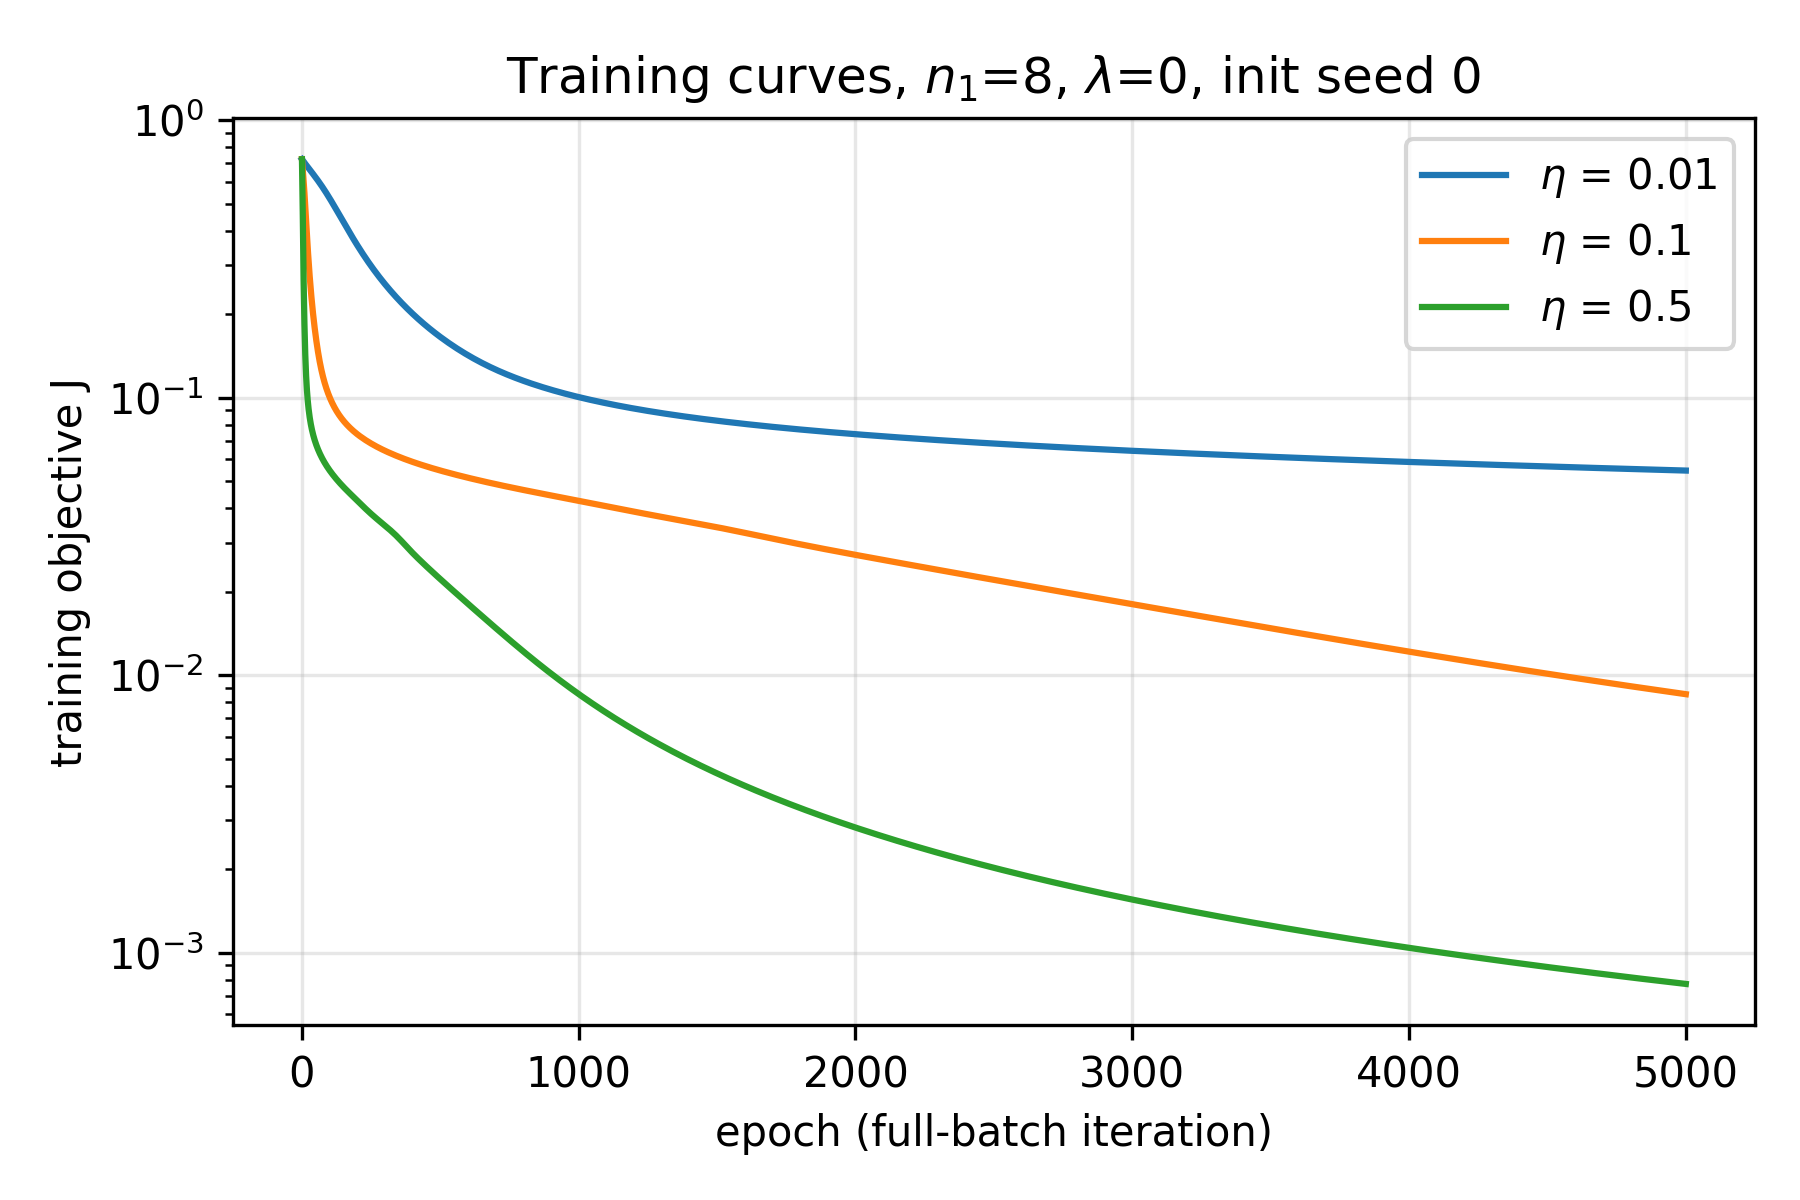
\includegraphics[width=0.85\linewidth]{../results/fig_loss_1.png}
  \caption{Training objective $J$ (logarithmic scale) against the epoch for $\eta=0.01$, $0.1$ and $0.5$. Reference configuration $n_1=8$, $\lambda=0$, initialization seed 0, which is not the selected configuration; training curves only. For all three learning rates $J$ decreases over the 5000 epochs, and at the epoch cap the curve for a larger $\eta$ lies lower.}
  \label{fig:loss}
\end{figure}

\begin{figure}[htbp]
  \centering
  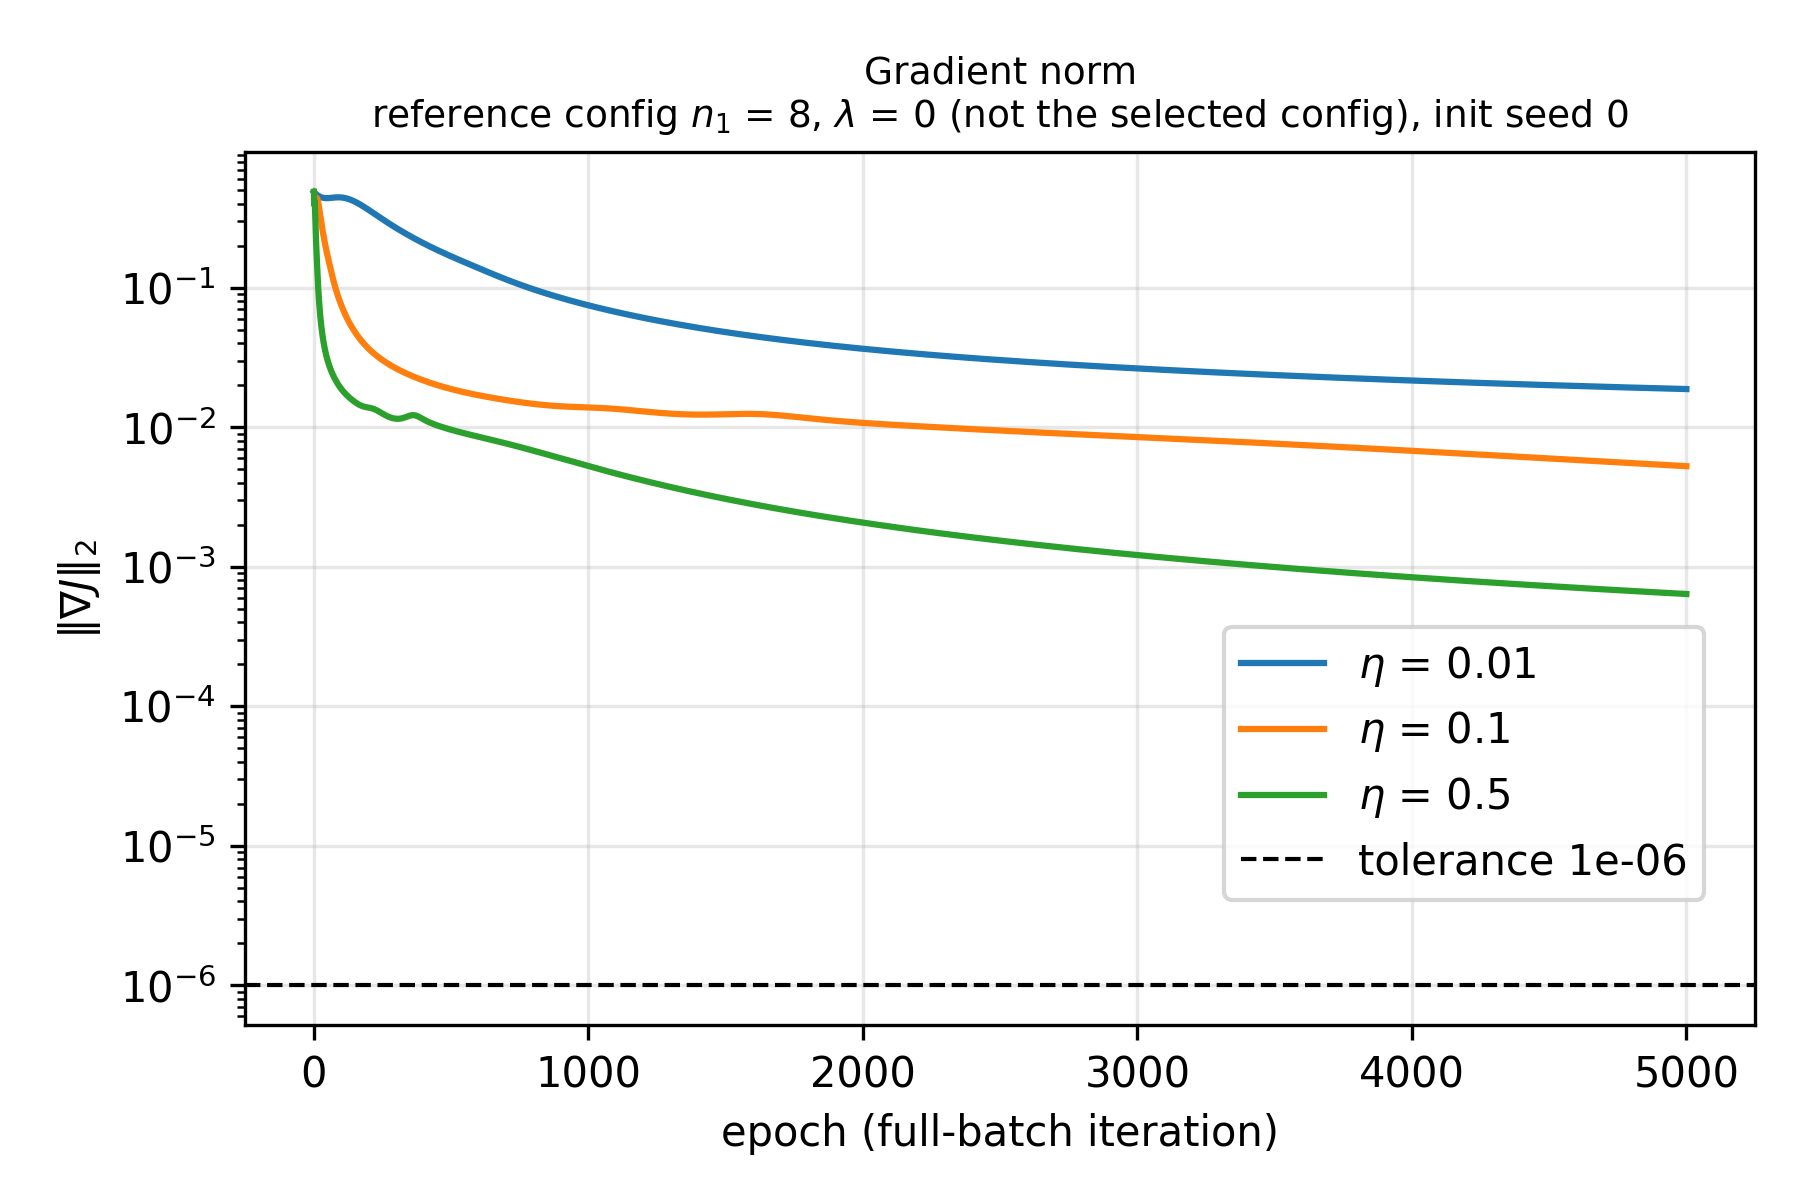
\includegraphics[width=0.85\linewidth]{../results/fig_gradnorm_2.png}
  \caption{Gradient norm $\lVert\nabla J\rVert_2$ (logarithmic scale) against the epoch for $\eta=0.01$, $0.1$ and $0.5$. Same reference configuration as Figure~\ref{fig:loss} ($n_1=8$, $\lambda=0$, seed 0; not the selected configuration); training curves only. The dashed line marks the tolerance $10^{-6}$, which none of the three curves reaches within 5000 epochs.}
  \label{fig:gradnorm}
\end{figure}

\begin{figure}[htbp]
  \centering
  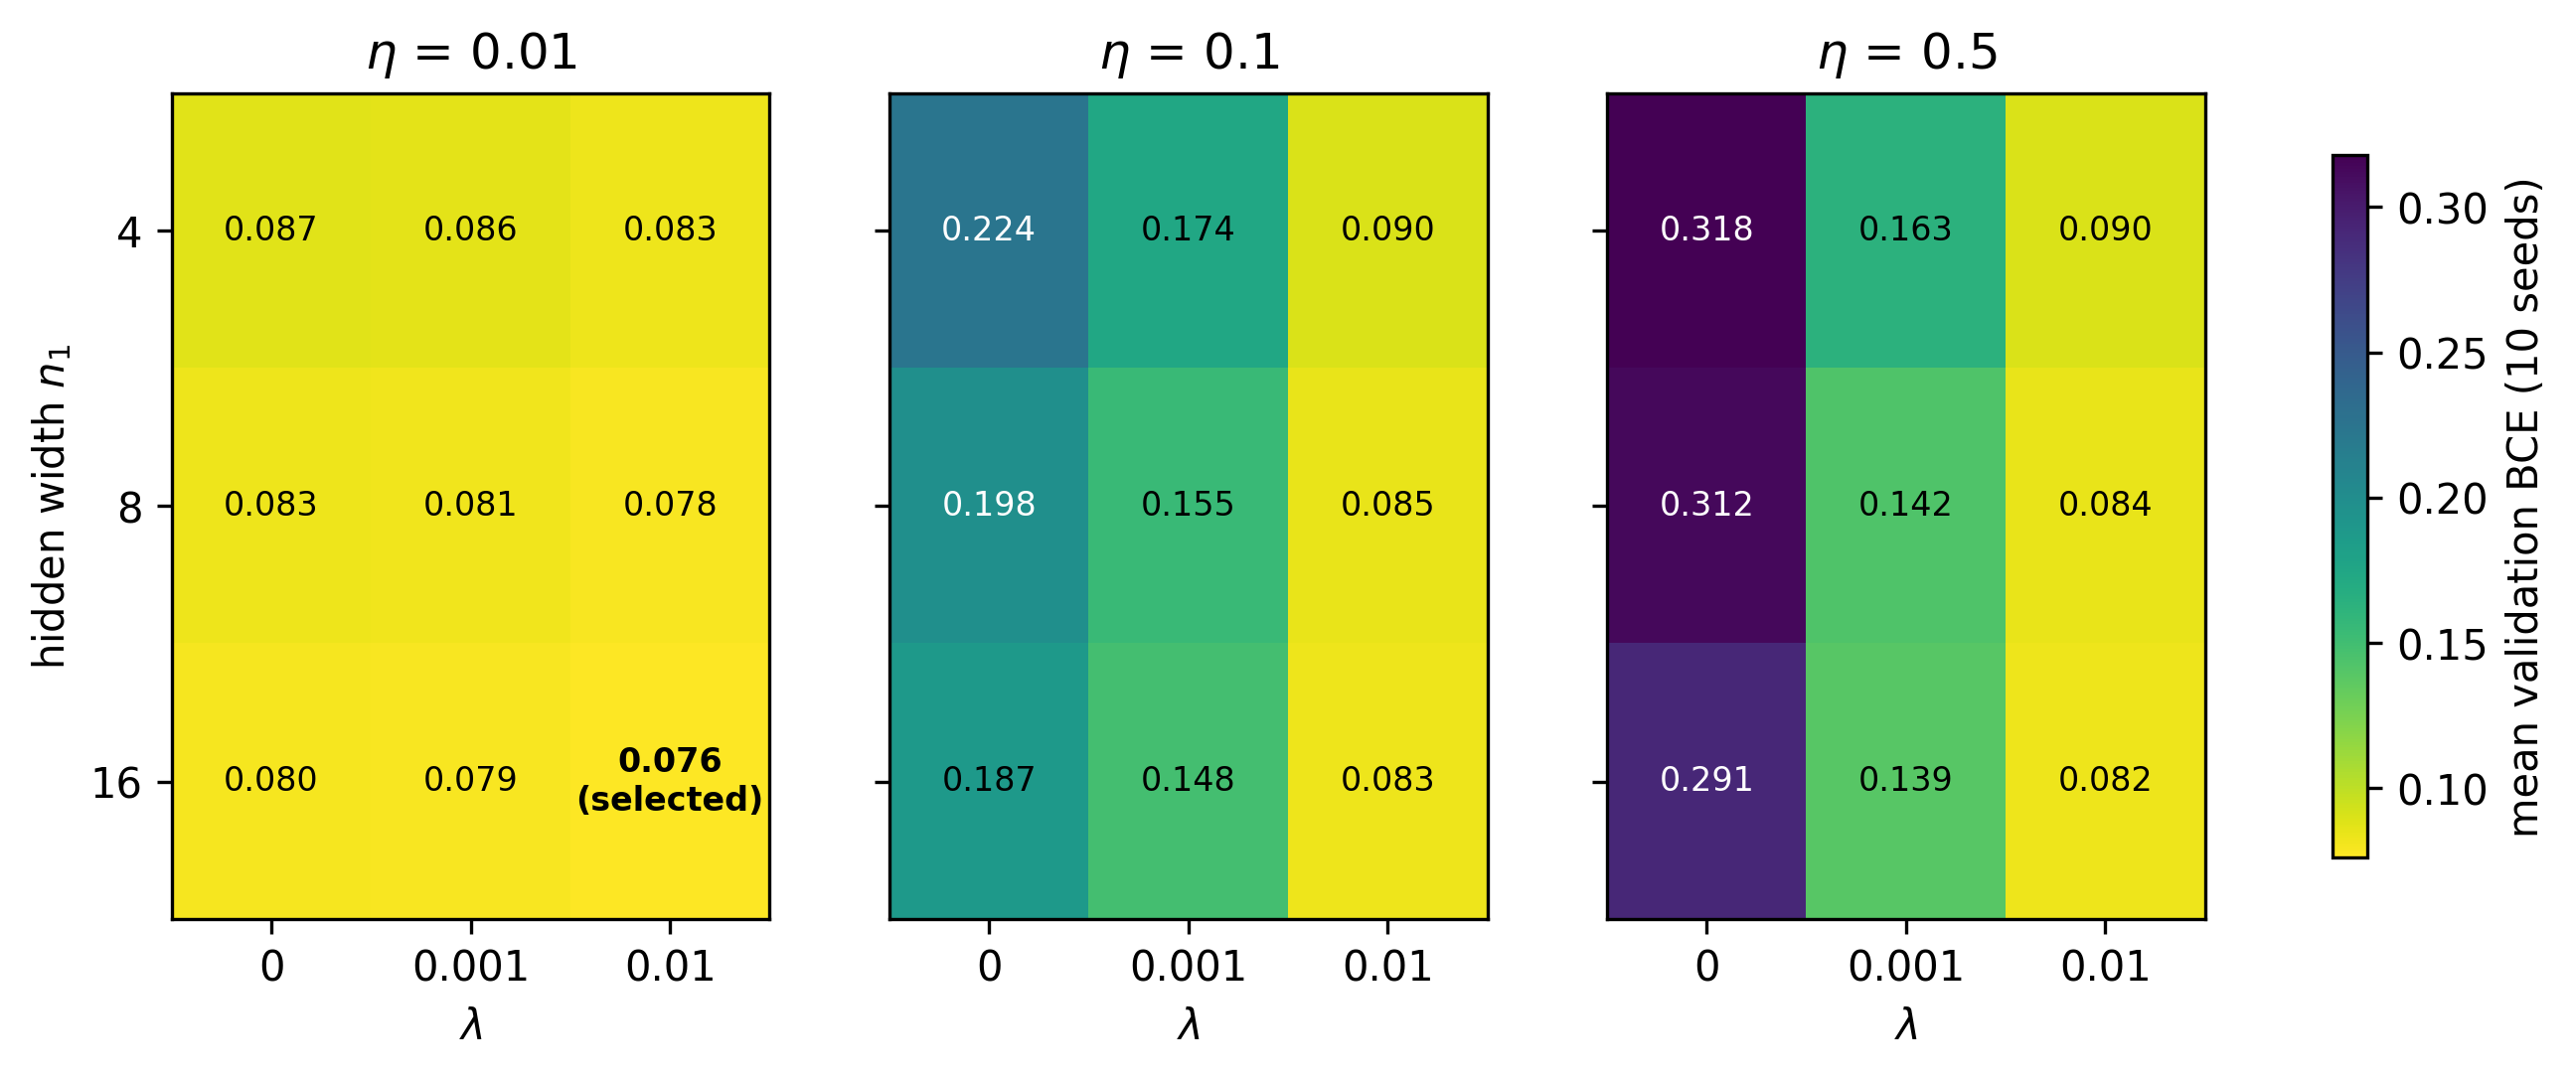
\includegraphics[width=\linewidth]{../results/fig_val_1.png}
  \caption{Mean validation BCE over initialization seeds 0--9 for each of the 27 grid cells, one panel per learning rate, with the hidden width $n_1$ on the vertical axis and $\lambda$ on the horizontal axis. The selected cell ($\eta=0.01$, $n_1=16$, $\lambda=0.01$) is marked.}
  \label{fig:val}
\end{figure}

\begin{figure}[htbp]
  \centering
  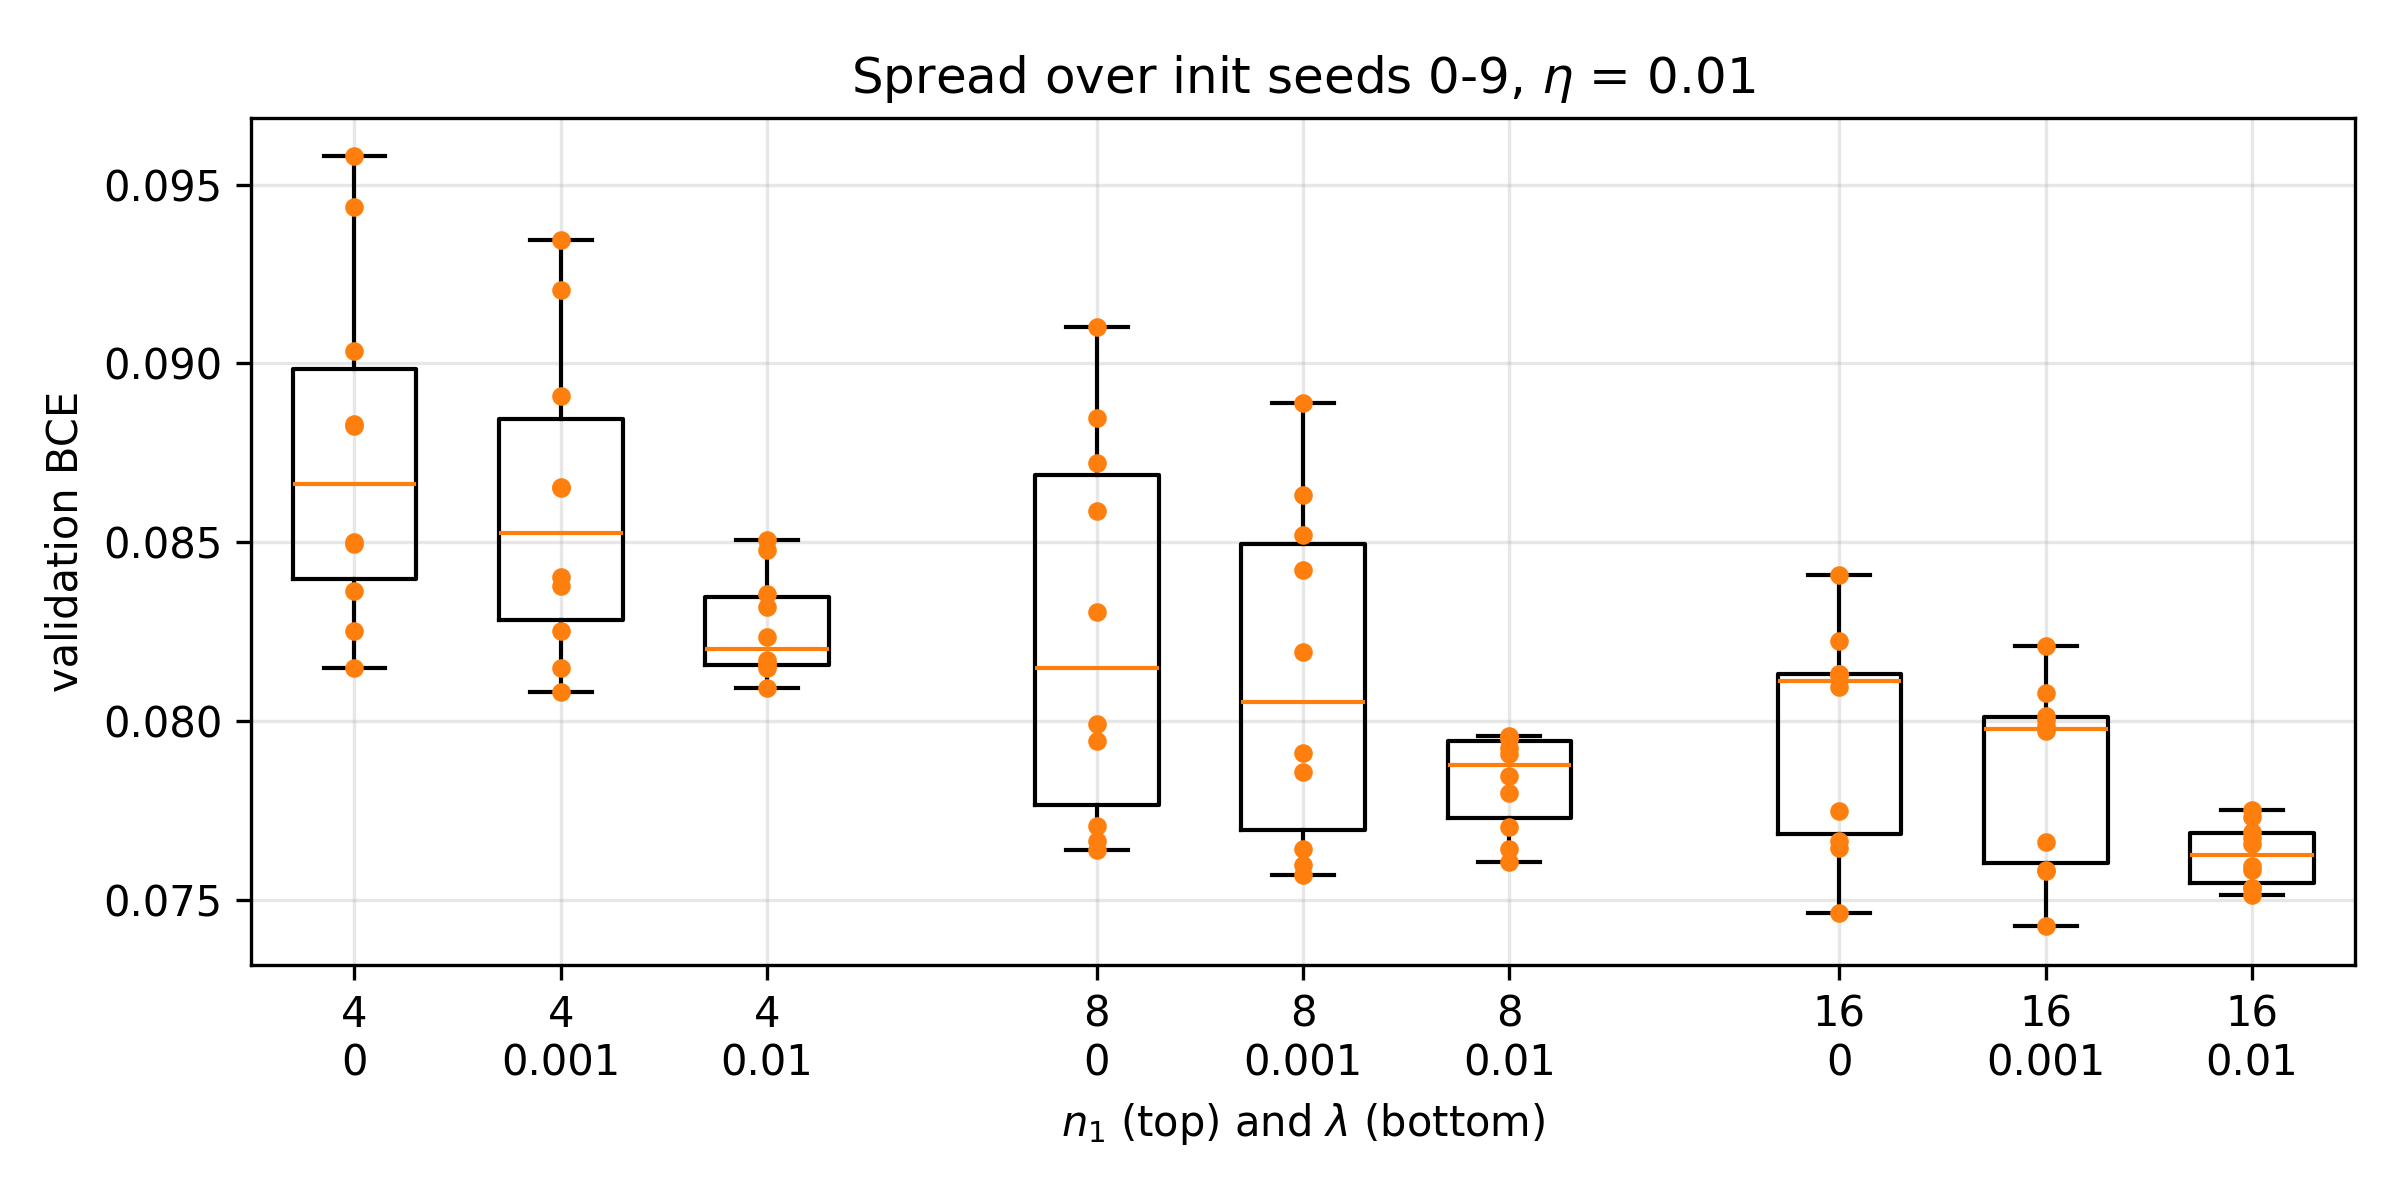
\includegraphics[width=\linewidth]{../results/fig_seeds_1.png}
  \caption{Validation BCE of the ten initialization seeds (points) and their box plots for the nine grid cells with $\eta=0.01$, labeled by $n_1$ (top) and $\lambda$ (bottom). For each hidden width, the spread over seeds is smallest at $\lambda=0.01$.}
  \label{fig:seeds}
\end{figure}

\begin{figure}[htbp]
  \centering
  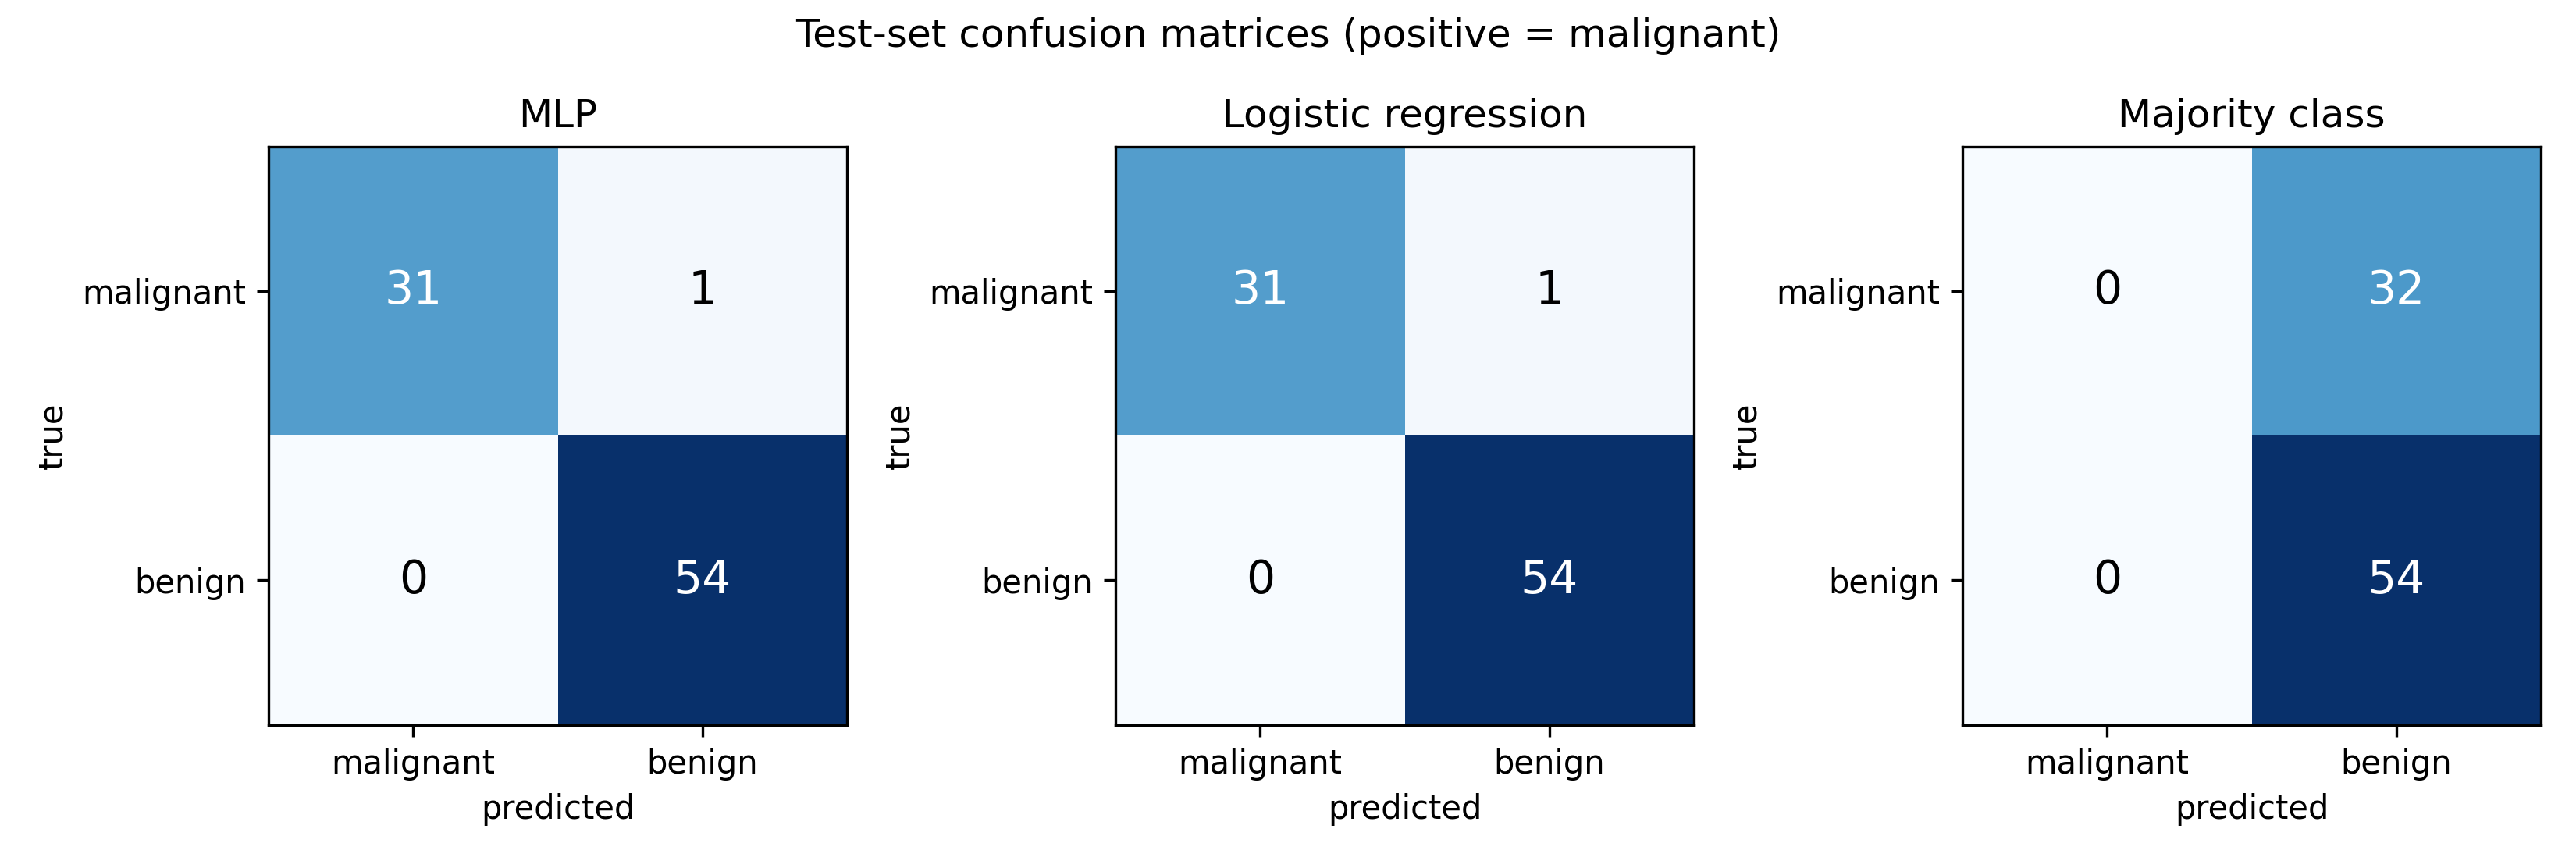
\includegraphics[width=\linewidth]{../results/fig_confusion_1.png}
  \caption{Test-set confusion matrices (positive class = malignant, threshold $0.5$) for the final MLP, logistic regression and the majority-class rule. The MLP and logistic regression have the same counts; the majority-class rule predicts benign for all 86 examples.}
  \label{fig:confusion}
\end{figure}

\begin{figure}[htbp]
  \centering
  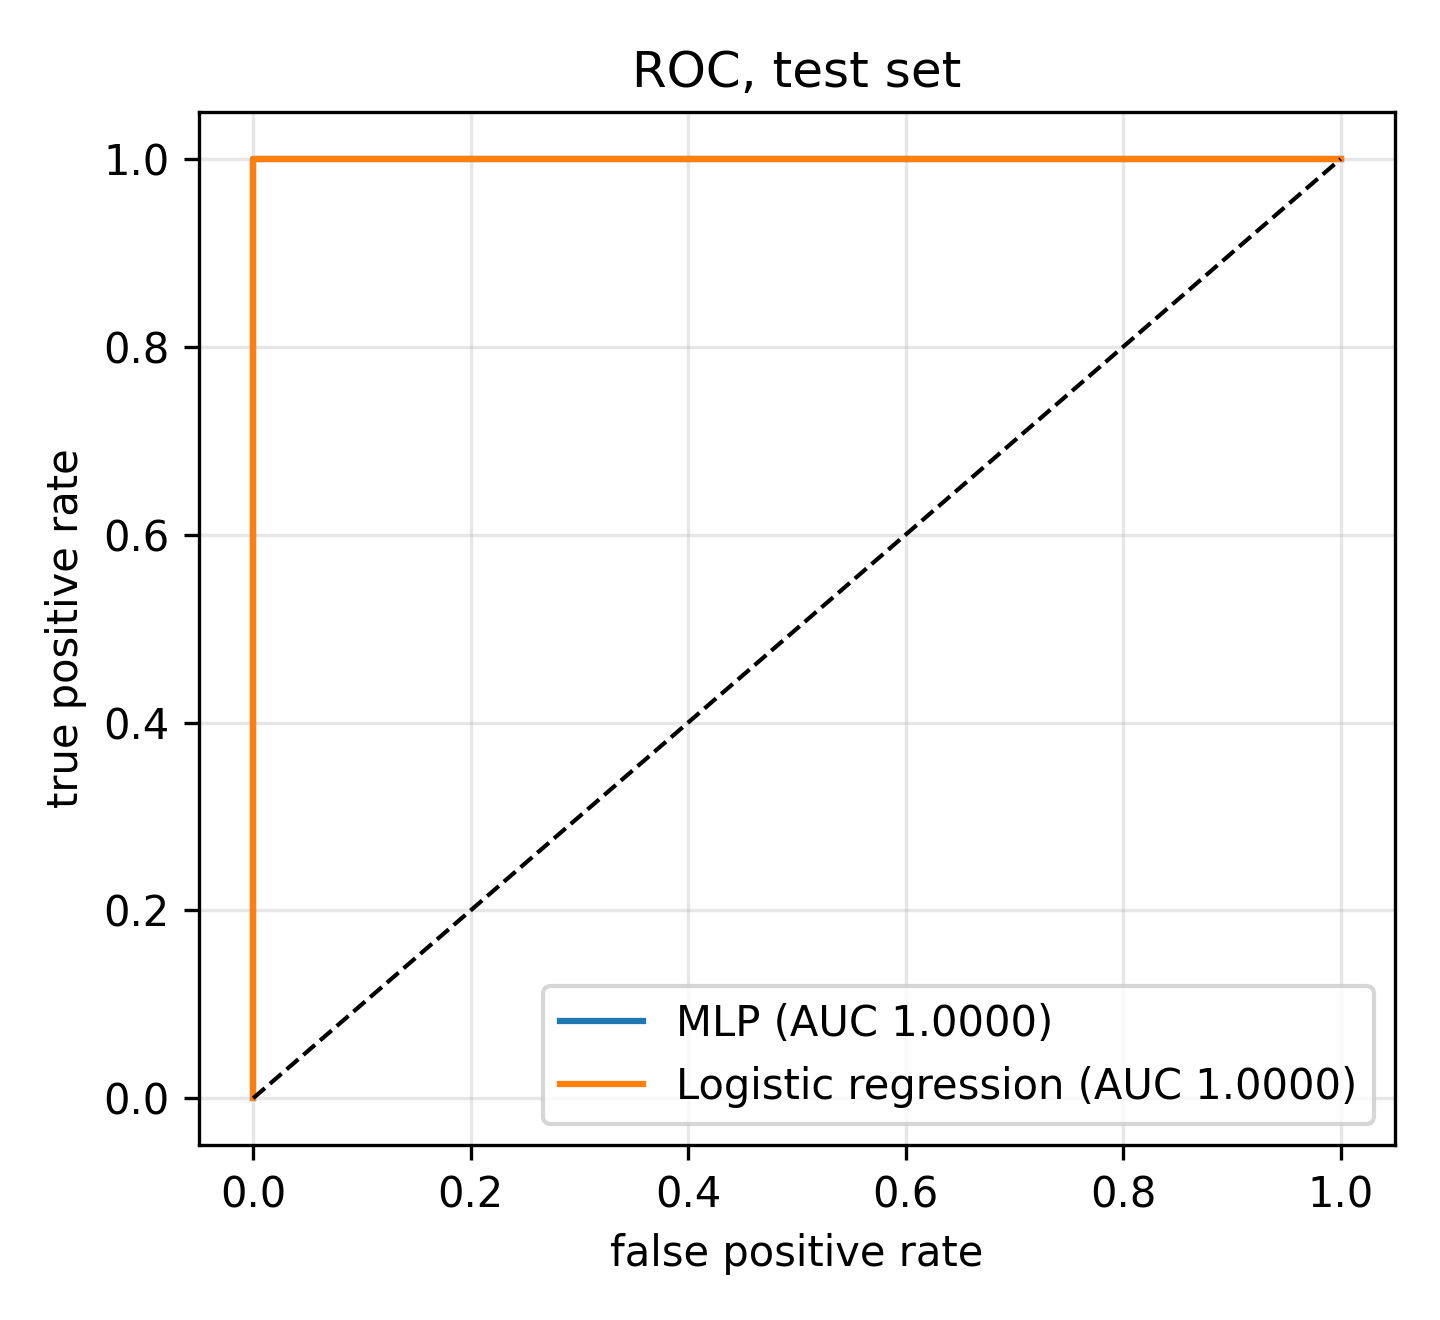
\includegraphics[width=0.6\linewidth]{../results/fig_roc_1.png}
  \caption{Test-set ROC curves of the final MLP and logistic regression; the two curves coincide and both have $\mathrm{AUC}=1.0$. An AUC of $1.0$ means a perfect ranking of the 86 test examples, not a perfect classifier: at the fixed threshold $0.5$ one malignant case is missed. The dotted diagonal corresponds to random ranking.}
  \label{fig:roc}
\end{figure}

\begin{figure}[htbp]
  \centering
  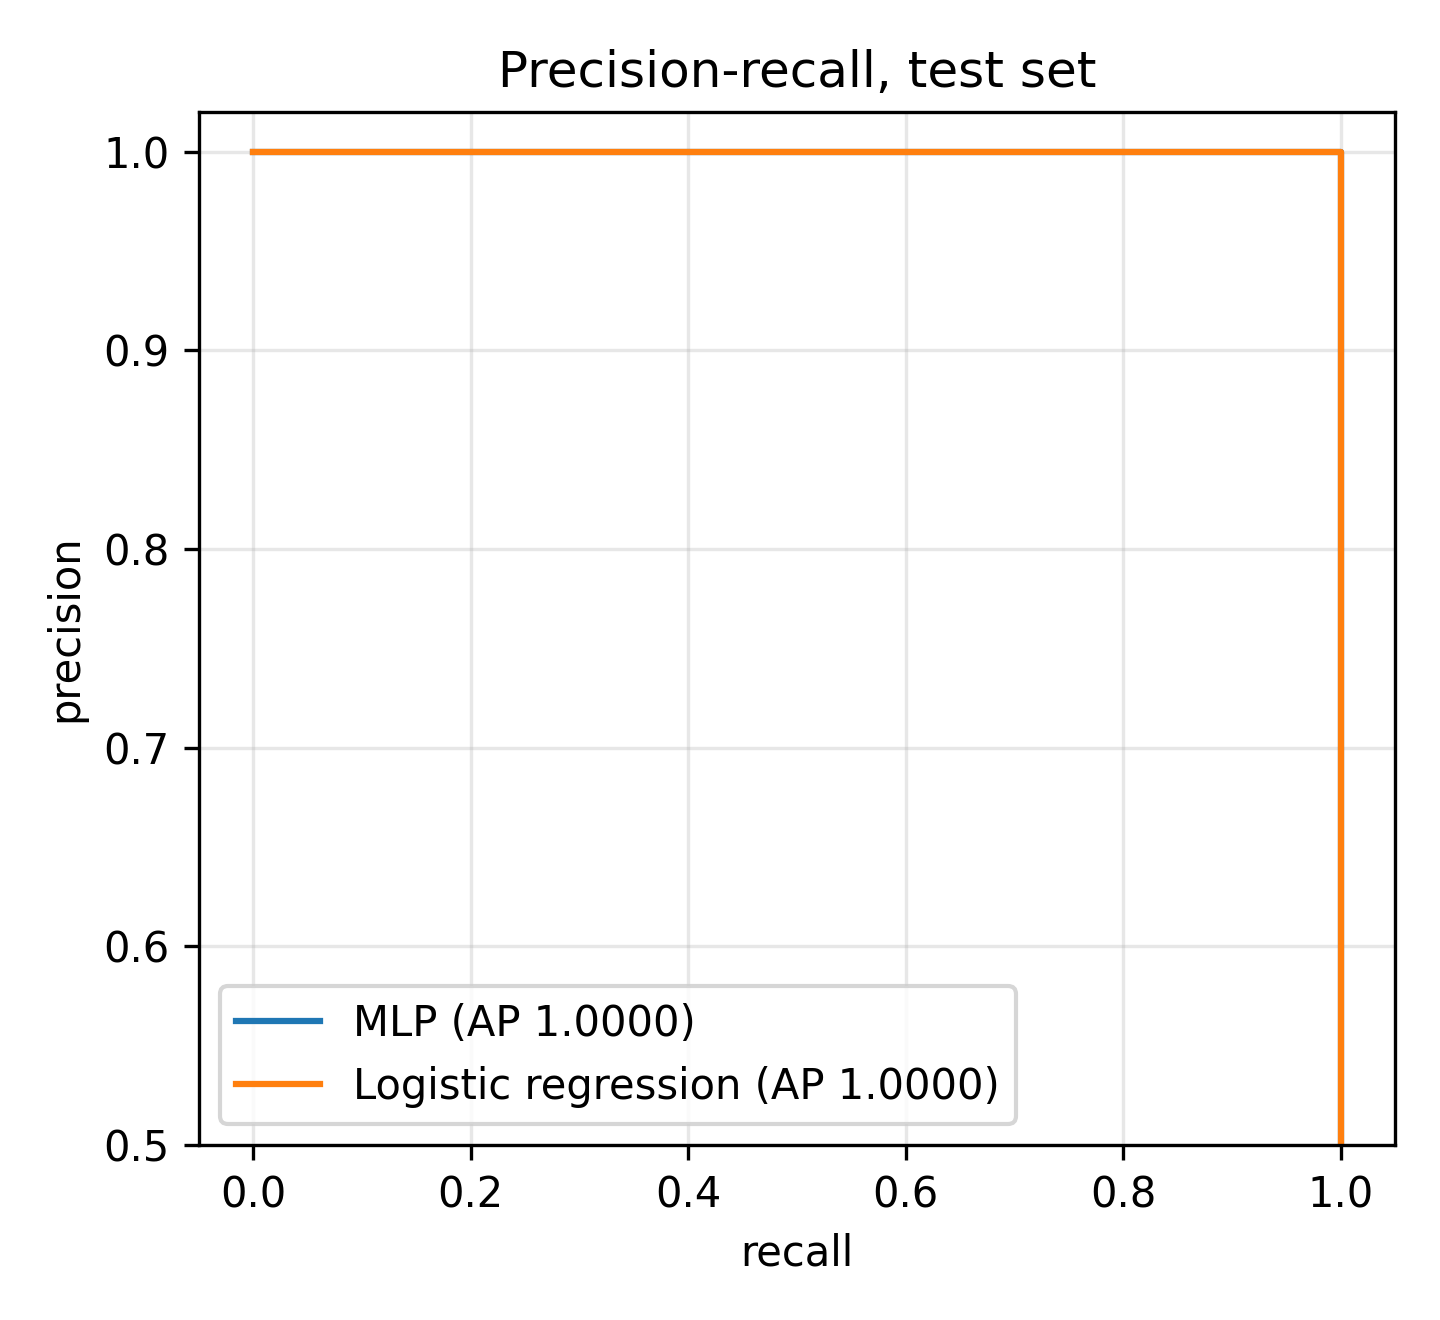
\includegraphics[width=0.6\linewidth]{../results/fig_pr_2.png}
  \caption{Test-set precision--recall curves of the final MLP and logistic regression; the two curves coincide and both have $\mathrm{AP}=1.0$. As for the ROC curve, this means a perfect ranking of the 86 test examples, not a perfect classifier: at the fixed threshold $0.5$ one malignant case is missed. The dotted line marks the fraction of malignant examples in the test set.}
  \label{fig:pr}
\end{figure}

\clearpage % place all tables and figures of Section 3.3 before Section 3.4

\subsection{Analysis and Discussion}
\label{sec:analysis}

\paragraph{Accuracy.}
On the 86 test examples the final MLP reaches an accuracy of $0.9884$, a precision of $1.0000$ and a recall of $0.9688$ (Table~\ref{tab:test}), against $0.6279$ for the majority-class rule. The single error is a false negative: a malignant mass that the model labels benign. In a screening-support setting this is the costlier kind of error, because a missed malignant case may delay follow-up, whereas a false alarm would lead to further examination. The missed case has $\hat p=0.4619$, just below the threshold $0.5$, and every malignant test example receives a higher $\hat p$ than every benign one (AUC $=1.0$). The ranking of the scores is therefore perfect on this test set, and the error comes from the fixed threshold. The threshold was not tuned.

\paragraph{Convergence and stability.}
In the reference configuration ($n_1=8$, $\lambda=0$, seed 0), the objective starts at $J=0.7230$ and decreases for all three learning rates. After 5000 epochs it is $0.054615$ for $\eta=0.01$, $0.008543$ for $\eta=0.1$ and $0.000772$ for $\eta=0.5$, with gradient norms $0.018799$, $0.005266$ and $0.000639$. A larger learning rate thus reaches a lower training objective within the same number of epochs, and none of the three runs diverged or reached the tolerance $10^{-6}$. The validation error tells a different story. With $\lambda=0$, the mean validation BCE rises with the learning rate, for example for $n_1=8$ from $0.08250$ at $\eta=0.01$ to $0.19755$ at $\eta=0.1$ and $0.31228$ at $\eta=0.5$. For $n_1=8$ and $\eta=0.5$ the mean training BCE is $0.00080$ against a validation BCE of $0.31228$. A training error far below the validation error is consistent with overfitting; this was not tested directly. Regularization narrows the gap: at $\eta=0.5$ and $\lambda=0.01$ the training BCE is $0.05715$ and the validation BCE $0.08441$, and the validation BCE over the three widths lies in $0.0825$--$0.0898$ for $\eta=0.1$ and $0.0824$--$0.0898$ for $\eta=0.5$, close to the range $0.0763$--$0.0826$ at $\eta=0.01$. The mean validation accuracy varies much less than the BCE, from $0.9471$ in the weakest cell to $0.9765$ for the selected configuration. The selected model did not reach the tolerance: it stopped at the 5000-epoch cap with $\lVert\nabla J\rVert_2=0.015658$, and only 6 of the 270 grid runs (all with $\eta=0.5$, $n_1=4$, $\lambda=0.01$) satisfied $\lVert\nabla J\rVert_2<10^{-6}$ before the cap.

\paragraph{Computational cost.}
The selected network has $P=513$ parameters (\eqref{eq:wdbc-params}; $129$ and $257$ for $n_1=4$ and $8$). Each epoch is one forward and one backward pass over the 398 training examples, and a run is limited to 5000 epochs. The grid consists of 270 such runs.

\paragraph{Comparison with the baseline.}
The MLP and logistic regression make the same single error (confusion counts $31/0/54/1$) and share all threshold-based metrics. The MLP has the lower test log loss, $0.0497$ against $0.0610$, but this is a difference between two values computed on 86 examples from one split, without an estimate of its uncertainty. We therefore claim no difference in quality between the two models. On this split, the added hidden layer did not change the classification of any test example relative to a linear model.

\paragraph{Limitations.}
The study uses one dataset of 569 samples, one split with 85 validation and 86 test examples, and no external validation. The data file has no patient identifiers, so a patient-level split was not possible, and the assumption that the examples are independent is not verified. The selected configuration sits on the edge of the grid on all three axes, so a setting with lower validation error may lie outside the grid. In addition, the small learning rate combined with the epoch cap may act like early stopping, because training ends while $J$ is still decreasing; part of the validation advantage of $\eta=0.01$ may therefore come from this. This is a possibility, not a tested explanation. The final model was evaluated once on the test set; a later seed-sensitivity check on the test set did not change it and was not used for any decision. In that check every initialization seed gave the same confusion counts $31/0/54/1$ and the test log loss ranged from $0.04864$ to $0.05022$, so the test result did not change across the ten seeds tried. Finally, this is an educational model and not a diagnostic tool; the results support no clinical claim.

\section{Conclusion}
\label{sec:concl}

We derived backpropagation for a one-hidden-layer perceptron with a sigmoid output and binary cross-entropy, implemented it from scratch in NumPy, and verified it: the analytic gradients agree with centered finite differences to within $2.1\times10^{-11}$. The learning rate, hidden width and regularization strength were chosen from a 27-cell grid by the mean validation loss over ten initialization seeds. The selected configuration ($\eta=0.01$, $n_1=16$, $\lambda=0.01$; mean validation BCE $0.076259$) lies on the edge of the grid on all three axes. Without regularization the validation loss grew with the learning rate, from $0.0796$--$0.0875$ at $\eta=0.01$ to $0.2906$--$0.3179$ at $\eta=0.5$, which is consistent with overfitting; with $\lambda=0.01$ the corresponding ranges were $0.0763$--$0.0826$ and $0.0824$--$0.0898$. The final model stopped at the 5000-epoch cap with a final gradient norm of $0.015658$. On the 86 test examples it reached an accuracy of $0.9884$, a precision of $1.0000$ and a recall of $0.9688$, with a test log loss of $0.0497$; it missed one of the 32 malignant cases.

The study is relevant as an illustration of how a classifier for fine-needle-aspirate features can be built, validated and judged, for example as a screening-support aid. It is an educational model; it is not a diagnostic tool, and the results support no clinical use. As for the method, the MLP matches logistic regression on this split: both make the same single error, and the majority-class rule reaches an accuracy of $0.6279$. The test log losses are $0.0497$ and $0.0610$, two values from 86 examples and one split, and we draw no stronger conclusion from them.

Several extensions were not done and are proposed as future work: (i) external validation on data from another source; (ii) patient-level or cross-validated splits, which would also give an uncertainty estimate for the test metrics; (iii) choosing the decision threshold on validation data to favor recall, since the missed case had $\hat p=0.4619$, just below the threshold $0.5$, a value that is a test-set observation and not a basis for changing the threshold; (iv) a grid that extends beyond the current edge in learning rate, width and regularization strength; and (v) mini-batch training in place of full-batch gradient descent.


\newpage
\addcontentsline{toc}{section}{References}
\emergencystretch=3em
\begin{thebibliography}{99}

\bibitem{boler2022}
Boler, A. K., Roy, S., Chakraborty, A., \& Bandyopadhyay, A. (2022). Reproducibility of the ``International Academy of Cytology Yokohama System for Reporting Breast Cytology'': A retrospective analysis of 70 cases. \textit{Journal of Cytology, 39}(4), 159--162. \url{https://doi.org/10.4103/joc.joc_203_21}

\bibitem{street1993}
Street, W. N., Wolberg, W. H., \& Mangasarian, O. L. (1993). Nuclear feature extraction for breast tumor diagnosis. \textit{Proceedings of SPIE, 1905}, 861--870. \url{https://doi.org/10.1117/12.148698}

\bibitem{wdbc}
Wolberg, W., Mangasarian, O., Street, N., \& Street, W. (1993). \textit{Breast Cancer Wisconsin (Diagnostic)} [Dataset]. UCI Machine Learning Repository. Retrieved October 26, 2026, from \url{https://doi.org/10.24432/C5DW2B}

\bibitem{who2026}
World Health Organization. (2026, July 3). \textit{Breast cancer} [Fact sheet]. Retrieved October 30, 2026, from \url{https://www.who.int/news-room/fact-sheets/detail/breast-cancer}

\bibitem{yu2012}
Yu, Y.-H., Wei, W., \& Liu, J.-L. (2012). Diagnostic value of fine-needle aspiration biopsy for breast mass: A systematic review and meta-analysis. \textit{BMC Cancer, 12}, Article 41. \url{https://doi.org/10.1186/1471-2407-12-41}

\end{thebibliography}

\end{document}
